\documentclass[twoside]{book}

% Packages required by doxygen
\usepackage{fixltx2e}
\usepackage{calc}
\usepackage{doxygen}
\usepackage[export]{adjustbox} % also loads graphicx
\usepackage{graphicx}
\usepackage[utf8]{inputenc}
\usepackage{makeidx}
\usepackage{multicol}
\usepackage{multirow}
\PassOptionsToPackage{warn}{textcomp}
\usepackage{textcomp}
\usepackage[nointegrals]{wasysym}
\usepackage[table]{xcolor}

% Font selection
\usepackage[T1]{fontenc}
\usepackage[scaled=.90]{helvet}
\usepackage{courier}
\usepackage{amssymb}
\usepackage{sectsty}
\renewcommand{\familydefault}{\sfdefault}
\allsectionsfont{%
  \fontseries{bc}\selectfont%
  \color{darkgray}%
}
\renewcommand{\DoxyLabelFont}{%
  \fontseries{bc}\selectfont%
  \color{darkgray}%
}
\newcommand{\+}{\discretionary{\mbox{\scriptsize$\hookleftarrow$}}{}{}}

% Page & text layout
\usepackage{geometry}
\geometry{%
  a4paper,%
  top=2.5cm,%
  bottom=2.5cm,%
  left=2.5cm,%
  right=2.5cm%
}
\tolerance=750
\hfuzz=15pt
\hbadness=750
\setlength{\emergencystretch}{15pt}
\setlength{\parindent}{0cm}
\setlength{\parskip}{3ex plus 2ex minus 2ex}
\makeatletter
\renewcommand{\paragraph}{%
  \@startsection{paragraph}{4}{0ex}{-1.0ex}{1.0ex}{%
    \normalfont\normalsize\bfseries\SS@parafont%
  }%
}
\renewcommand{\subparagraph}{%
  \@startsection{subparagraph}{5}{0ex}{-1.0ex}{1.0ex}{%
    \normalfont\normalsize\bfseries\SS@subparafont%
  }%
}
\makeatother

% Headers & footers
\usepackage{fancyhdr}
\pagestyle{fancyplain}
\fancyhead[LE]{\fancyplain{}{\bfseries\thepage}}
\fancyhead[CE]{\fancyplain{}{}}
\fancyhead[RE]{\fancyplain{}{\bfseries\leftmark}}
\fancyhead[LO]{\fancyplain{}{\bfseries\rightmark}}
\fancyhead[CO]{\fancyplain{}{}}
\fancyhead[RO]{\fancyplain{}{\bfseries\thepage}}
\fancyfoot[LE]{\fancyplain{}{}}
\fancyfoot[CE]{\fancyplain{}{}}
\fancyfoot[RE]{\fancyplain{}{\bfseries\scriptsize Generated by Doxygen }}
\fancyfoot[LO]{\fancyplain{}{\bfseries\scriptsize Generated by Doxygen }}
\fancyfoot[CO]{\fancyplain{}{}}
\fancyfoot[RO]{\fancyplain{}{}}
\renewcommand{\footrulewidth}{0.4pt}
\renewcommand{\chaptermark}[1]{%
  \markboth{#1}{}%
}
\renewcommand{\sectionmark}[1]{%
  \markright{\thesection\ #1}%
}

% Indices & bibliography
\usepackage{natbib}
\usepackage[titles]{tocloft}
\setcounter{tocdepth}{3}
\setcounter{secnumdepth}{5}
\makeindex

% Hyperlinks (required, but should be loaded last)
\usepackage{ifpdf}
\ifpdf
  \usepackage[pdftex,pagebackref=true]{hyperref}
\else
  \usepackage[ps2pdf,pagebackref=true]{hyperref}
\fi
\hypersetup{%
  colorlinks=true,%
  linkcolor=blue,%
  citecolor=blue,%
  unicode%
}

% Custom commands
\newcommand{\clearemptydoublepage}{%
  \newpage{\pagestyle{empty}\cleardoublepage}%
}

\usepackage{caption}
\captionsetup{labelsep=space,justification=centering,font={bf},singlelinecheck=off,skip=4pt,position=top}

%===== C O N T E N T S =====

\begin{document}

% Titlepage & ToC
\hypersetup{pageanchor=false,
             bookmarksnumbered=true,
             pdfencoding=unicode
            }
\pagenumbering{alph}
\begin{titlepage}
\vspace*{7cm}
\begin{center}%
{\Large My Project }\\
\vspace*{1cm}
{\large Generated by Doxygen 1.8.13}\\
\end{center}
\end{titlepage}
\clearemptydoublepage
\pagenumbering{roman}
\tableofcontents
\clearemptydoublepage
\pagenumbering{arabic}
\hypersetup{pageanchor=true}

%--- Begin generated contents ---
\chapter{Logic Assignment 2}
\label{md_README}
\Hypertarget{md_README}
Submission for Assignment 2 of CS F214 -\/ Logic in CS, 2018-\/19.

\subsection*{Running}

Start by running the {\ttfamily Logic} file (precompiled) in a Linux terminal.

\subsection*{Features}


\begin{DoxyItemize}
\item Modularized code, separated into various files.
\item Namespaces for constants so as to not pollute the global namespace.
\item Well documented, including time complexities of every function.
\item Performance and stress tested, to see the limits of the program.
\end{DoxyItemize}

\subsubsection*{Part 1}


\begin{DoxyItemize}
\item Convert an infix expression to postfix form
\item Convert a postfix expression to a Binary Parse Tree
\item Convert a Binary Parse Tree to infix expression
\end{DoxyItemize}

\subsubsection*{Part 2}


\begin{DoxyItemize}
\item Check validity of a given proof in propositional logic with a limited set of rules
\begin{DoxyItemize}
\item Premise
\item And introduction
\item And elimination
\item Or introduction
\item Implication eliminiation
\item Modus Tollens
\end{DoxyItemize}
\item We convert the formula of each line to its parse tree, and then compare the inorder strings of previous proof lines as required by the rule.
\end{DoxyItemize}

\subsection*{Assumptions and Performance Testing}

\subsubsection*{Part 1}


\begin{DoxyItemize}
\item We assume that the given formula of only contains propositional atoms made up of the 26 lowercase English alphabets, and that it is well formed propositional formula.
\item We have implemented a operator priority based approach to resolve ambiguity in case the formula is not well parenthesized.
\end{DoxyItemize}

\paragraph*{Memory}

  Crashed (2819 atoms)\+: 

\subsubsection*{Part 2}

\paragraph*{Memory}



\subsection*{Tools used}


\begin{DoxyItemize}
\item Editors and I\+D\+Es\+: Sublime Text, Vim, C\+Lion
\item Compilers\+: gcc and cmake
\item Performance test\+: valgrind
\item Documentation\+: doxygen
\item Version Control\+: git, with a repo hosted at local gitlab \href{https://td.bits-hyderabad.ac.in/lab/mach64/logic-assgn-2/}\texttt{ server}.
\end{DoxyItemize}

\subsection*{Contributors}


\begin{DoxyItemize}
\item \href{f20170184@hyderabad.bits-pilani.ac.in}\texttt{ Krut Patel}
\item \href{f20170130@hyderabad.bits-pilani.ac.in}\texttt{ Niral Khambhati} 
\end{DoxyItemize}
\chapter{Namespace Index}
\section{Namespace List}
Here is a list of all namespaces with brief descriptions\+:\begin{DoxyCompactList}
\item\contentsline{section}{\mbox{\hyperlink{namespaceoperators}{operators}} \\*Defining operators using namespace to make it easy for changing input syntax as and when required }{\pageref{namespaceoperators}}{}
\item\contentsline{section}{\mbox{\hyperlink{namespacerule__literals}{rule\+\_\+literals}} \\*Defining types of rules for ease of making changes if required }{\pageref{namespacerule__literals}}{}
\item\contentsline{section}{\mbox{\hyperlink{namespacetest__gen}{test\+\_\+gen}} }{\pageref{namespacetest__gen}}{}
\item\contentsline{section}{\mbox{\hyperlink{namespaceverbs}{verbs}} \\*Defining verbs for ease of making changes if required }{\pageref{namespaceverbs}}{}
\end{DoxyCompactList}

\chapter{Class Index}
\section{Class List}
Here are the classes, structs, unions and interfaces with brief descriptions\+:\begin{DoxyCompactList}
\item\contentsline{section}{\hyperlink{classBTree}{B\+Tree} }{\pageref{classBTree}}{}
\item\contentsline{section}{\hyperlink{classProofLine}{Proof\+Line} }{\pageref{classProofLine}}{}
\end{DoxyCompactList}

\chapter{File Index}
\section{File List}
Here is a list of all files with brief descriptions\+:\begin{DoxyCompactList}
\item\contentsline{section}{\hyperlink{BTree_8cpp}{B\+Tree.\+cpp} }{\pageref{BTree_8cpp}}{}
\item\contentsline{section}{\hyperlink{BTree_8h}{B\+Tree.\+h} }{\pageref{BTree_8h}}{}
\item\contentsline{section}{\hyperlink{main_8cpp}{main.\+cpp} }{\pageref{main_8cpp}}{}
\item\contentsline{section}{\hyperlink{operators_8cpp}{operators.\+cpp} }{\pageref{operators_8cpp}}{}
\item\contentsline{section}{\hyperlink{operators_8h}{operators.\+h} }{\pageref{operators_8h}}{}
\item\contentsline{section}{\hyperlink{rules_8cpp}{rules.\+cpp} }{\pageref{rules_8cpp}}{}
\item\contentsline{section}{\hyperlink{rules_8h}{rules.\+h} }{\pageref{rules_8h}}{}
\item\contentsline{section}{\hyperlink{task1_8cpp}{task1.\+cpp} }{\pageref{task1_8cpp}}{}
\item\contentsline{section}{\hyperlink{task1_8h}{task1.\+h} }{\pageref{task1_8h}}{}
\item\contentsline{section}{\hyperlink{task2_8cpp}{task2.\+cpp} }{\pageref{task2_8cpp}}{}
\item\contentsline{section}{\hyperlink{task2_8h}{task2.\+h} }{\pageref{task2_8h}}{}
\end{DoxyCompactList}

\chapter{Namespace Documentation}
\hypertarget{namespaceoperators}{}\section{operators Namespace Reference}
\label{namespaceoperators}\index{operators@{operators}}


Defining operators using namespace to make it easy for changing input syntax as and when required.  


\subsection*{Variables}
\begin{DoxyCompactItemize}
\item 
const char \mbox{\hyperlink{namespaceoperators_abc0d09c09b437de98007962a590ea557}{N\+EG}} \{\textquotesingle{}$\sim$\textquotesingle{}\}
\begin{DoxyCompactList}\small\item\em Defines N\+E\+G\+A\+T\+I\+ON. \end{DoxyCompactList}\item 
const char \mbox{\hyperlink{namespaceoperators_aff9dc11d489d31278c1e3f90ae09dd9b}{A\+ND}} \{\textquotesingle{}$^\wedge$\textquotesingle{}\}
\begin{DoxyCompactList}\small\item\em Defines A\+ND. \end{DoxyCompactList}\item 
const char \mbox{\hyperlink{namespaceoperators_a1f469207e0d08770fc7bbac128cfd845}{OR}} \{\textquotesingle{}V\textquotesingle{}\}
\begin{DoxyCompactList}\small\item\em Defines OR. \end{DoxyCompactList}\item 
const char \mbox{\hyperlink{namespaceoperators_a40fe490f326324304d4529854fb2deea}{I\+M\+PL}} \{\textquotesingle{}$>$\textquotesingle{}\}
\begin{DoxyCompactList}\small\item\em Defines I\+M\+P\+L\+I\+C\+A\+T\+I\+ON. \end{DoxyCompactList}\end{DoxyCompactItemize}


\subsection{Detailed Description}
Defining operators using namespace to make it easy for changing input syntax as and when required. 

\subsection{Variable Documentation}
\mbox{\Hypertarget{namespaceoperators_abc0d09c09b437de98007962a590ea557}\label{namespaceoperators_abc0d09c09b437de98007962a590ea557}} 
\index{operators@{operators}!N\+EG@{N\+EG}}
\index{N\+EG@{N\+EG}!operators@{operators}}
\subsubsection{\texorpdfstring{N\+EG}{NEG}}
{\footnotesize\ttfamily const char operators\+::\+N\+EG \{\textquotesingle{}$\sim$\textquotesingle{}\}}



Defines N\+E\+G\+A\+T\+I\+ON. 

\mbox{\Hypertarget{namespaceoperators_aff9dc11d489d31278c1e3f90ae09dd9b}\label{namespaceoperators_aff9dc11d489d31278c1e3f90ae09dd9b}} 
\index{operators@{operators}!A\+ND@{A\+ND}}
\index{A\+ND@{A\+ND}!operators@{operators}}
\subsubsection{\texorpdfstring{A\+ND}{AND}}
{\footnotesize\ttfamily const char operators\+::\+A\+ND \{\textquotesingle{}$^\wedge$\textquotesingle{}\}}



Defines A\+ND. 

\mbox{\Hypertarget{namespaceoperators_a1f469207e0d08770fc7bbac128cfd845}\label{namespaceoperators_a1f469207e0d08770fc7bbac128cfd845}} 
\index{operators@{operators}!OR@{OR}}
\index{OR@{OR}!operators@{operators}}
\subsubsection{\texorpdfstring{OR}{OR}}
{\footnotesize\ttfamily const char operators\+::\+OR \{\textquotesingle{}V\textquotesingle{}\}}



Defines OR. 

\mbox{\Hypertarget{namespaceoperators_a40fe490f326324304d4529854fb2deea}\label{namespaceoperators_a40fe490f326324304d4529854fb2deea}} 
\index{operators@{operators}!I\+M\+PL@{I\+M\+PL}}
\index{I\+M\+PL@{I\+M\+PL}!operators@{operators}}
\subsubsection{\texorpdfstring{I\+M\+PL}{IMPL}}
{\footnotesize\ttfamily const char operators\+::\+I\+M\+PL \{\textquotesingle{}$>$\textquotesingle{}\}}



Defines I\+M\+P\+L\+I\+C\+A\+T\+I\+ON. 


\hypertarget{namespacerule__literals}{}\section{rule\+\_\+literals Namespace Reference}
\label{namespacerule__literals}\index{rule\+\_\+literals@{rule\+\_\+literals}}


Defining types of rules for ease of making changes if required.  


\subsection*{Variables}
\begin{DoxyCompactItemize}
\item 
const std\+::string \mbox{\hyperlink{namespacerule__literals_a28f9829b438b28638be8c82c450237e1}{P\+R\+EM}} \{\char`\"{}P\char`\"{}\}
\begin{DoxyCompactList}\small\item\em $<$ Enables us to use A\+ND, OR, I\+M\+PL, N\+EG \end{DoxyCompactList}\item 
const std\+::string \mbox{\hyperlink{namespacerule__literals_a94631d6e4135b29c6bacb5cde1d9719b}{A\+N\+D\+\_\+I}} \{A\+ND, \mbox{\hyperlink{namespaceverbs_a160cd2b49b96eb11b6db907bf94b5c3a}{verbs\+::\+I\+N\+T\+RO}}\}
\begin{DoxyCompactList}\small\item\em Defines A\+ND I\+N\+T\+R\+O\+D\+U\+C\+T\+I\+ON. \end{DoxyCompactList}\item 
const std\+::string \mbox{\hyperlink{namespacerule__literals_af7751bceefaea1ff69733140731b7770}{A\+N\+D\+\_\+\+E1}} \{A\+ND, \mbox{\hyperlink{namespaceverbs_ae28355cc9321ebee9abcd23bb6e1b836}{verbs\+::\+E\+L\+IM}}, \textquotesingle{}1\textquotesingle{}\}
\begin{DoxyCompactList}\small\item\em Defines A\+ND E\+L\+I\+M\+I\+N\+A\+T\+I\+ON 1. \end{DoxyCompactList}\item 
const std\+::string \mbox{\hyperlink{namespacerule__literals_a0861b2e3104a4c1465d3dbbb362b5d10}{A\+N\+D\+\_\+\+E2}} \{A\+ND, \mbox{\hyperlink{namespaceverbs_ae28355cc9321ebee9abcd23bb6e1b836}{verbs\+::\+E\+L\+IM}}, \textquotesingle{}2\textquotesingle{}\}
\begin{DoxyCompactList}\small\item\em Defines A\+ND E\+L\+I\+M\+I\+N\+A\+T\+I\+ON 2. \end{DoxyCompactList}\item 
const std\+::string \mbox{\hyperlink{namespacerule__literals_a0c61940a6e12e4ea3a41346b5b3c5870}{O\+R\+\_\+\+I1}} \{OR, \mbox{\hyperlink{namespaceverbs_a160cd2b49b96eb11b6db907bf94b5c3a}{verbs\+::\+I\+N\+T\+RO}}, \textquotesingle{}1\textquotesingle{}\}
\begin{DoxyCompactList}\small\item\em Defines OR I\+N\+T\+R\+O\+D\+U\+C\+T\+I\+ON 1. \end{DoxyCompactList}\item 
const std\+::string \mbox{\hyperlink{namespacerule__literals_a2c1ef10ddec67801c44ea5b3e15ed133}{O\+R\+\_\+\+I2}} \{OR, \mbox{\hyperlink{namespaceverbs_a160cd2b49b96eb11b6db907bf94b5c3a}{verbs\+::\+I\+N\+T\+RO}}, \textquotesingle{}2\textquotesingle{}\}
\begin{DoxyCompactList}\small\item\em Defines OR I\+N\+T\+R\+O\+D\+U\+C\+T\+I\+ON 2. \end{DoxyCompactList}\item 
const std\+::string \mbox{\hyperlink{namespacerule__literals_a51a002ead2192c49b9c6216c5fbe3b74}{I\+M\+P\+L\+\_\+E}} \{I\+M\+PL, \mbox{\hyperlink{namespaceverbs_ae28355cc9321ebee9abcd23bb6e1b836}{verbs\+::\+E\+L\+IM}}\}
\begin{DoxyCompactList}\small\item\em Defines I\+M\+P\+L\+I\+ES E\+L\+I\+M\+I\+N\+A\+T\+I\+ON. \end{DoxyCompactList}\item 
const std\+::string \mbox{\hyperlink{namespacerule__literals_a056c3d0c0b701c07f444b7c5adfa8ff4}{MT}} \{\char`\"{}MT\char`\"{}\}
\begin{DoxyCompactList}\small\item\em Defines M\+O\+D\+US T\+O\+L\+L\+E\+NS. \end{DoxyCompactList}\end{DoxyCompactItemize}


\subsection{Detailed Description}
Defining types of rules for ease of making changes if required. 

\subsection{Variable Documentation}
\mbox{\Hypertarget{namespacerule__literals_a28f9829b438b28638be8c82c450237e1}\label{namespacerule__literals_a28f9829b438b28638be8c82c450237e1}} 
\index{rule\+\_\+literals@{rule\+\_\+literals}!P\+R\+EM@{P\+R\+EM}}
\index{P\+R\+EM@{P\+R\+EM}!rule\+\_\+literals@{rule\+\_\+literals}}
\subsubsection{\texorpdfstring{P\+R\+EM}{PREM}}
{\footnotesize\ttfamily const std\+::string rule\+\_\+literals\+::\+P\+R\+EM \{\char`\"{}P\char`\"{}\}}



$<$ Enables us to use A\+ND, OR, I\+M\+PL, N\+EG 

Defines P\+R\+E\+M\+I\+SE \mbox{\Hypertarget{namespacerule__literals_a94631d6e4135b29c6bacb5cde1d9719b}\label{namespacerule__literals_a94631d6e4135b29c6bacb5cde1d9719b}} 
\index{rule\+\_\+literals@{rule\+\_\+literals}!A\+N\+D\+\_\+I@{A\+N\+D\+\_\+I}}
\index{A\+N\+D\+\_\+I@{A\+N\+D\+\_\+I}!rule\+\_\+literals@{rule\+\_\+literals}}
\subsubsection{\texorpdfstring{A\+N\+D\+\_\+I}{AND\_I}}
{\footnotesize\ttfamily const std\+::string rule\+\_\+literals\+::\+A\+N\+D\+\_\+I \{A\+ND, \mbox{\hyperlink{namespaceverbs_a160cd2b49b96eb11b6db907bf94b5c3a}{verbs\+::\+I\+N\+T\+RO}}\}}



Defines A\+ND I\+N\+T\+R\+O\+D\+U\+C\+T\+I\+ON. 

\mbox{\Hypertarget{namespacerule__literals_af7751bceefaea1ff69733140731b7770}\label{namespacerule__literals_af7751bceefaea1ff69733140731b7770}} 
\index{rule\+\_\+literals@{rule\+\_\+literals}!A\+N\+D\+\_\+\+E1@{A\+N\+D\+\_\+\+E1}}
\index{A\+N\+D\+\_\+\+E1@{A\+N\+D\+\_\+\+E1}!rule\+\_\+literals@{rule\+\_\+literals}}
\subsubsection{\texorpdfstring{A\+N\+D\+\_\+\+E1}{AND\_E1}}
{\footnotesize\ttfamily const std\+::string rule\+\_\+literals\+::\+A\+N\+D\+\_\+\+E1 \{A\+ND, \mbox{\hyperlink{namespaceverbs_ae28355cc9321ebee9abcd23bb6e1b836}{verbs\+::\+E\+L\+IM}}, \textquotesingle{}1\textquotesingle{}\}}



Defines A\+ND E\+L\+I\+M\+I\+N\+A\+T\+I\+ON 1. 

\mbox{\Hypertarget{namespacerule__literals_a0861b2e3104a4c1465d3dbbb362b5d10}\label{namespacerule__literals_a0861b2e3104a4c1465d3dbbb362b5d10}} 
\index{rule\+\_\+literals@{rule\+\_\+literals}!A\+N\+D\+\_\+\+E2@{A\+N\+D\+\_\+\+E2}}
\index{A\+N\+D\+\_\+\+E2@{A\+N\+D\+\_\+\+E2}!rule\+\_\+literals@{rule\+\_\+literals}}
\subsubsection{\texorpdfstring{A\+N\+D\+\_\+\+E2}{AND\_E2}}
{\footnotesize\ttfamily const std\+::string rule\+\_\+literals\+::\+A\+N\+D\+\_\+\+E2 \{A\+ND, \mbox{\hyperlink{namespaceverbs_ae28355cc9321ebee9abcd23bb6e1b836}{verbs\+::\+E\+L\+IM}}, \textquotesingle{}2\textquotesingle{}\}}



Defines A\+ND E\+L\+I\+M\+I\+N\+A\+T\+I\+ON 2. 

\mbox{\Hypertarget{namespacerule__literals_a0c61940a6e12e4ea3a41346b5b3c5870}\label{namespacerule__literals_a0c61940a6e12e4ea3a41346b5b3c5870}} 
\index{rule\+\_\+literals@{rule\+\_\+literals}!O\+R\+\_\+\+I1@{O\+R\+\_\+\+I1}}
\index{O\+R\+\_\+\+I1@{O\+R\+\_\+\+I1}!rule\+\_\+literals@{rule\+\_\+literals}}
\subsubsection{\texorpdfstring{O\+R\+\_\+\+I1}{OR\_I1}}
{\footnotesize\ttfamily const std\+::string rule\+\_\+literals\+::\+O\+R\+\_\+\+I1 \{OR, \mbox{\hyperlink{namespaceverbs_a160cd2b49b96eb11b6db907bf94b5c3a}{verbs\+::\+I\+N\+T\+RO}}, \textquotesingle{}1\textquotesingle{}\}}



Defines OR I\+N\+T\+R\+O\+D\+U\+C\+T\+I\+ON 1. 

\mbox{\Hypertarget{namespacerule__literals_a2c1ef10ddec67801c44ea5b3e15ed133}\label{namespacerule__literals_a2c1ef10ddec67801c44ea5b3e15ed133}} 
\index{rule\+\_\+literals@{rule\+\_\+literals}!O\+R\+\_\+\+I2@{O\+R\+\_\+\+I2}}
\index{O\+R\+\_\+\+I2@{O\+R\+\_\+\+I2}!rule\+\_\+literals@{rule\+\_\+literals}}
\subsubsection{\texorpdfstring{O\+R\+\_\+\+I2}{OR\_I2}}
{\footnotesize\ttfamily const std\+::string rule\+\_\+literals\+::\+O\+R\+\_\+\+I2 \{OR, \mbox{\hyperlink{namespaceverbs_a160cd2b49b96eb11b6db907bf94b5c3a}{verbs\+::\+I\+N\+T\+RO}}, \textquotesingle{}2\textquotesingle{}\}}



Defines OR I\+N\+T\+R\+O\+D\+U\+C\+T\+I\+ON 2. 

\mbox{\Hypertarget{namespacerule__literals_a51a002ead2192c49b9c6216c5fbe3b74}\label{namespacerule__literals_a51a002ead2192c49b9c6216c5fbe3b74}} 
\index{rule\+\_\+literals@{rule\+\_\+literals}!I\+M\+P\+L\+\_\+E@{I\+M\+P\+L\+\_\+E}}
\index{I\+M\+P\+L\+\_\+E@{I\+M\+P\+L\+\_\+E}!rule\+\_\+literals@{rule\+\_\+literals}}
\subsubsection{\texorpdfstring{I\+M\+P\+L\+\_\+E}{IMPL\_E}}
{\footnotesize\ttfamily const std\+::string rule\+\_\+literals\+::\+I\+M\+P\+L\+\_\+E \{I\+M\+PL, \mbox{\hyperlink{namespaceverbs_ae28355cc9321ebee9abcd23bb6e1b836}{verbs\+::\+E\+L\+IM}}\}}



Defines I\+M\+P\+L\+I\+ES E\+L\+I\+M\+I\+N\+A\+T\+I\+ON. 

\mbox{\Hypertarget{namespacerule__literals_a056c3d0c0b701c07f444b7c5adfa8ff4}\label{namespacerule__literals_a056c3d0c0b701c07f444b7c5adfa8ff4}} 
\index{rule\+\_\+literals@{rule\+\_\+literals}!MT@{MT}}
\index{MT@{MT}!rule\+\_\+literals@{rule\+\_\+literals}}
\subsubsection{\texorpdfstring{MT}{MT}}
{\footnotesize\ttfamily const std\+::string rule\+\_\+literals\+::\+MT \{\char`\"{}MT\char`\"{}\}}



Defines M\+O\+D\+US T\+O\+L\+L\+E\+NS. 


\hypertarget{namespaceverbs}{}\section{verbs Namespace Reference}
\label{namespaceverbs}\index{verbs@{verbs}}
\subsection*{Variables}
\begin{DoxyCompactItemize}
\item 
const char \hyperlink{namespaceverbs_a160cd2b49b96eb11b6db907bf94b5c3a}{I\+N\+T\+RO} = \textquotesingle{}i\textquotesingle{}
\item 
const char \hyperlink{namespaceverbs_ae28355cc9321ebee9abcd23bb6e1b836}{E\+L\+IM} = \textquotesingle{}e\textquotesingle{}
\end{DoxyCompactItemize}


\subsection{Variable Documentation}
\mbox{\Hypertarget{namespaceverbs_ae28355cc9321ebee9abcd23bb6e1b836}\label{namespaceverbs_ae28355cc9321ebee9abcd23bb6e1b836}} 
\index{verbs@{verbs}!E\+L\+IM@{E\+L\+IM}}
\index{E\+L\+IM@{E\+L\+IM}!verbs@{verbs}}
\subsubsection{\texorpdfstring{E\+L\+IM}{ELIM}}
{\footnotesize\ttfamily const char verbs\+::\+E\+L\+IM = \textquotesingle{}e\textquotesingle{}}

\mbox{\Hypertarget{namespaceverbs_a160cd2b49b96eb11b6db907bf94b5c3a}\label{namespaceverbs_a160cd2b49b96eb11b6db907bf94b5c3a}} 
\index{verbs@{verbs}!I\+N\+T\+RO@{I\+N\+T\+RO}}
\index{I\+N\+T\+RO@{I\+N\+T\+RO}!verbs@{verbs}}
\subsubsection{\texorpdfstring{I\+N\+T\+RO}{INTRO}}
{\footnotesize\ttfamily const char verbs\+::\+I\+N\+T\+RO = \textquotesingle{}i\textquotesingle{}}


\chapter{Class Documentation}
\hypertarget{classBTree}{}\section{B\+Tree Class Reference}
\label{classBTree}\index{B\+Tree@{B\+Tree}}


Class to represent a Binary Tree.  




{\ttfamily \#include $<$B\+Tree.\+h$>$}



Collaboration diagram for B\+Tree\+:\nopagebreak
\begin{figure}[H]
\begin{center}
\leavevmode
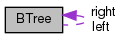
\includegraphics[width=163pt]{classBTree__coll__graph}
\end{center}
\end{figure}
\subsection*{Public Member Functions}
\begin{DoxyCompactItemize}
\item 
\mbox{\hyperlink{classBTree_a816ccfed62d3bd439b61c03f660d1cc6}{B\+Tree}} (char \mbox{\hyperlink{classBTree_a3d5016b19ab621d5c61cf633ec012a72}{token}})
\begin{DoxyCompactList}\small\item\em Constructor for creating a \mbox{\hyperlink{classBTree}{B\+Tree}} object. \end{DoxyCompactList}\item 
\mbox{\hyperlink{classBTree_a1d0dbad21ec825a7c8e5625709010e6c}{$\sim$\+B\+Tree}} ()
\begin{DoxyCompactList}\small\item\em Destructor for given binary tree. \end{DoxyCompactList}\item 
void \mbox{\hyperlink{classBTree_ae80b1f2b89c404206d76e5371c820d7a}{add\+\_\+left\+\_\+child}} (\mbox{\hyperlink{classBTree}{B\+Tree}} $\ast$\mbox{\hyperlink{classBTree_ad7e7d928a099c40fbd0d323f76d7cf18}{left}})
\begin{DoxyCompactList}\small\item\em A function to assign left \mbox{\hyperlink{classBTree}{B\+Tree}} pointer. \end{DoxyCompactList}\item 
void \mbox{\hyperlink{classBTree_a03ed2114a3f21b5f1b6b0ae93d7cdc91}{add\+\_\+right\+\_\+child}} (\mbox{\hyperlink{classBTree}{B\+Tree}} $\ast$\mbox{\hyperlink{classBTree_af95770a535a9278b37fd73d7b6ae7f5e}{right}})
\begin{DoxyCompactList}\small\item\em A function to assign right \mbox{\hyperlink{classBTree}{B\+Tree}} pointer. \end{DoxyCompactList}\item 
std\+::string \mbox{\hyperlink{classBTree_a408f4bcf02423637c7132bcc44646f01}{get\+\_\+inorder}} ()
\begin{DoxyCompactList}\small\item\em A function for traversing the parse tree inorder. \end{DoxyCompactList}\end{DoxyCompactItemize}
\subsection*{Public Attributes}
\begin{DoxyCompactItemize}
\item 
char \mbox{\hyperlink{classBTree_a3d5016b19ab621d5c61cf633ec012a72}{token}}
\begin{DoxyCompactList}\small\item\em Char containing data for current node in binary tree. \end{DoxyCompactList}\item 
\mbox{\hyperlink{classBTree}{B\+Tree}} $\ast$ \mbox{\hyperlink{classBTree_ad7e7d928a099c40fbd0d323f76d7cf18}{left}}
\begin{DoxyCompactList}\small\item\em Pointer to left node in binary tree. \end{DoxyCompactList}\item 
\mbox{\hyperlink{classBTree}{B\+Tree}} $\ast$ \mbox{\hyperlink{classBTree_af95770a535a9278b37fd73d7b6ae7f5e}{right}}
\begin{DoxyCompactList}\small\item\em Pointer to right node in binary tree. \end{DoxyCompactList}\end{DoxyCompactItemize}
\subsection*{Related Functions}
(Note that these are not member functions.) \begin{DoxyCompactItemize}
\item 
std\+::string \mbox{\hyperlink{classBTree_a2dbc497c79c44fc43579cedee34296e8}{infix\+\_\+to\+\_\+postfix}} (std\+::string infix\+\_\+exp)
\begin{DoxyCompactList}\small\item\em Converts the infix expression to postfix. \end{DoxyCompactList}\item 
\mbox{\hyperlink{classBTree}{B\+Tree}} $\ast$ \mbox{\hyperlink{classBTree_a628ffca8bc269400217fa849038b6684}{postfix\+\_\+to\+\_\+parse\+\_\+tree}} (std\+::string $\ast$postfix)
\begin{DoxyCompactList}\small\item\em Generates a binary tree using given postfix expression. \end{DoxyCompactList}\item 
std\+::string \mbox{\hyperlink{classBTree_a9804f1d5620990cac8ac016f30cb6f4f}{parse\+\_\+tree\+\_\+to\+\_\+infix}} (\mbox{\hyperlink{classBTree}{B\+Tree}} $\ast$root)
\begin{DoxyCompactList}\small\item\em Traverses a given tree to produce corresponding infix expression. \end{DoxyCompactList}\end{DoxyCompactItemize}


\subsection{Detailed Description}
Class to represent a Binary Tree. 

This will be used to store the parse tree of the propositional formulas 

\subsection{Constructor \& Destructor Documentation}
\mbox{\Hypertarget{classBTree_a816ccfed62d3bd439b61c03f660d1cc6}\label{classBTree_a816ccfed62d3bd439b61c03f660d1cc6}} 
\index{B\+Tree@{B\+Tree}!B\+Tree@{B\+Tree}}
\index{B\+Tree@{B\+Tree}!B\+Tree@{B\+Tree}}
\subsubsection{\texorpdfstring{B\+Tree()}{BTree()}}
{\footnotesize\ttfamily B\+Tree\+::\+B\+Tree (\begin{DoxyParamCaption}\item[{char}]{token }\end{DoxyParamCaption})\hspace{0.3cm}{\ttfamily [explicit]}}



Constructor for creating a \mbox{\hyperlink{classBTree}{B\+Tree}} object. 

Complexity\+: O(1) 
\begin{DoxyParams}[1]{Parameters}
\mbox{\texttt{ in}}  & {\em token} & Character using which a new \mbox{\hyperlink{classBTree}{B\+Tree}} object will be created \\
\hline
\end{DoxyParams}
\mbox{\Hypertarget{classBTree_a1d0dbad21ec825a7c8e5625709010e6c}\label{classBTree_a1d0dbad21ec825a7c8e5625709010e6c}} 
\index{B\+Tree@{B\+Tree}!````~B\+Tree@{$\sim$\+B\+Tree}}
\index{````~B\+Tree@{$\sim$\+B\+Tree}!B\+Tree@{B\+Tree}}
\subsubsection{\texorpdfstring{$\sim$\+B\+Tree()}{~BTree()}}
{\footnotesize\ttfamily B\+Tree\+::$\sim$\+B\+Tree (\begin{DoxyParamCaption}{ }\end{DoxyParamCaption})}



Destructor for given binary tree. 

Complexity\+: O(1) 

\subsection{Member Function Documentation}
\mbox{\Hypertarget{classBTree_ae80b1f2b89c404206d76e5371c820d7a}\label{classBTree_ae80b1f2b89c404206d76e5371c820d7a}} 
\index{B\+Tree@{B\+Tree}!add\+\_\+left\+\_\+child@{add\+\_\+left\+\_\+child}}
\index{add\+\_\+left\+\_\+child@{add\+\_\+left\+\_\+child}!B\+Tree@{B\+Tree}}
\subsubsection{\texorpdfstring{add\+\_\+left\+\_\+child()}{add\_left\_child()}}
{\footnotesize\ttfamily void B\+Tree\+::add\+\_\+left\+\_\+child (\begin{DoxyParamCaption}\item[{\mbox{\hyperlink{classBTree}{B\+Tree}} $\ast$}]{left }\end{DoxyParamCaption})}



A function to assign left \mbox{\hyperlink{classBTree}{B\+Tree}} pointer. 

Complexity\+: O(1) 
\begin{DoxyParams}[1]{Parameters}
\mbox{\texttt{ in}}  & {\em left} & The pointer to \mbox{\hyperlink{classBTree}{B\+Tree}} object which has to be assigned \\
\hline
\end{DoxyParams}
\mbox{\Hypertarget{classBTree_a03ed2114a3f21b5f1b6b0ae93d7cdc91}\label{classBTree_a03ed2114a3f21b5f1b6b0ae93d7cdc91}} 
\index{B\+Tree@{B\+Tree}!add\+\_\+right\+\_\+child@{add\+\_\+right\+\_\+child}}
\index{add\+\_\+right\+\_\+child@{add\+\_\+right\+\_\+child}!B\+Tree@{B\+Tree}}
\subsubsection{\texorpdfstring{add\+\_\+right\+\_\+child()}{add\_right\_child()}}
{\footnotesize\ttfamily void B\+Tree\+::add\+\_\+right\+\_\+child (\begin{DoxyParamCaption}\item[{\mbox{\hyperlink{classBTree}{B\+Tree}} $\ast$}]{right }\end{DoxyParamCaption})}



A function to assign right \mbox{\hyperlink{classBTree}{B\+Tree}} pointer. 

Complexity\+: O(1) 
\begin{DoxyParams}[1]{Parameters}
\mbox{\texttt{ in}}  & {\em right} & The pointer to \mbox{\hyperlink{classBTree}{B\+Tree}} object which has to be assigned \\
\hline
\end{DoxyParams}
\mbox{\Hypertarget{classBTree_a408f4bcf02423637c7132bcc44646f01}\label{classBTree_a408f4bcf02423637c7132bcc44646f01}} 
\index{B\+Tree@{B\+Tree}!get\+\_\+inorder@{get\+\_\+inorder}}
\index{get\+\_\+inorder@{get\+\_\+inorder}!B\+Tree@{B\+Tree}}
\subsubsection{\texorpdfstring{get\+\_\+inorder()}{get\_inorder()}}
{\footnotesize\ttfamily std\+::string B\+Tree\+::get\+\_\+inorder (\begin{DoxyParamCaption}{ }\end{DoxyParamCaption})}



A function for traversing the parse tree inorder. 

Complexity\+: O(number of nodes in tree) on first run; O(1) on subsequent calls \begin{DoxyReturn}{Returns}
A string with infix expression without brackets 
\end{DoxyReturn}


\subsection{Friends And Related Function Documentation}
\mbox{\Hypertarget{classBTree_a2dbc497c79c44fc43579cedee34296e8}\label{classBTree_a2dbc497c79c44fc43579cedee34296e8}} 
\index{B\+Tree@{B\+Tree}!infix\+\_\+to\+\_\+postfix@{infix\+\_\+to\+\_\+postfix}}
\index{infix\+\_\+to\+\_\+postfix@{infix\+\_\+to\+\_\+postfix}!B\+Tree@{B\+Tree}}
\subsubsection{\texorpdfstring{infix\+\_\+to\+\_\+postfix()}{infix\_to\_postfix()}}
{\footnotesize\ttfamily std\+::string infix\+\_\+to\+\_\+postfix (\begin{DoxyParamCaption}\item[{std\+::string}]{infix\+\_\+exp }\end{DoxyParamCaption})\hspace{0.3cm}{\ttfamily [related]}}



Converts the infix expression to postfix. 

Complexity\+: O(number of characters in infix expression) 
\begin{DoxyParams}[1]{Parameters}
\mbox{\texttt{ in}}  & {\em infix\+\_\+exp} & The user-\/given string expression in infix form \\
\hline
\end{DoxyParams}
\begin{DoxyReturn}{Returns}
A string in postfix form 
\end{DoxyReturn}
\mbox{\Hypertarget{classBTree_a628ffca8bc269400217fa849038b6684}\label{classBTree_a628ffca8bc269400217fa849038b6684}} 
\index{B\+Tree@{B\+Tree}!postfix\+\_\+to\+\_\+parse\+\_\+tree@{postfix\+\_\+to\+\_\+parse\+\_\+tree}}
\index{postfix\+\_\+to\+\_\+parse\+\_\+tree@{postfix\+\_\+to\+\_\+parse\+\_\+tree}!B\+Tree@{B\+Tree}}
\subsubsection{\texorpdfstring{postfix\+\_\+to\+\_\+parse\+\_\+tree()}{postfix\_to\_parse\_tree()}}
{\footnotesize\ttfamily \mbox{\hyperlink{classBTree}{B\+Tree}} $\ast$ postfix\+\_\+to\+\_\+parse\+\_\+tree (\begin{DoxyParamCaption}\item[{std\+::string $\ast$}]{postfix }\end{DoxyParamCaption})\hspace{0.3cm}{\ttfamily [related]}}



Generates a binary tree using given postfix expression. 

\begin{DoxyWarning}{Warning}
This function modifies the postfix string it takes as argument!
\end{DoxyWarning}
Complexity\+: O(number of characters in postfix expression) 
\begin{DoxyParams}[1]{Parameters}
\mbox{\texttt{ in,out}}  & {\em postfix} & Postfix expression which we want to parse \\
\hline
\end{DoxyParams}
\begin{DoxyReturn}{Returns}
Root of the binary tree generated 
\end{DoxyReturn}
\mbox{\Hypertarget{classBTree_a9804f1d5620990cac8ac016f30cb6f4f}\label{classBTree_a9804f1d5620990cac8ac016f30cb6f4f}} 
\index{B\+Tree@{B\+Tree}!parse\+\_\+tree\+\_\+to\+\_\+infix@{parse\+\_\+tree\+\_\+to\+\_\+infix}}
\index{parse\+\_\+tree\+\_\+to\+\_\+infix@{parse\+\_\+tree\+\_\+to\+\_\+infix}!B\+Tree@{B\+Tree}}
\subsubsection{\texorpdfstring{parse\+\_\+tree\+\_\+to\+\_\+infix()}{parse\_tree\_to\_infix()}}
{\footnotesize\ttfamily std\+::string parse\+\_\+tree\+\_\+to\+\_\+infix (\begin{DoxyParamCaption}\item[{\mbox{\hyperlink{classBTree}{B\+Tree}} $\ast$}]{root }\end{DoxyParamCaption})\hspace{0.3cm}{\ttfamily [related]}}



Traverses a given tree to produce corresponding infix expression. 

Complexity\+: O(number of nodes in parse tree) 
\begin{DoxyParams}[1]{Parameters}
\mbox{\texttt{ in}}  & {\em root} & Root of binary tree to be traversed \\
\hline
\end{DoxyParams}
\begin{DoxyReturn}{Returns}
A string of infix expression of binary tree 
\end{DoxyReturn}


\subsection{Member Data Documentation}
\mbox{\Hypertarget{classBTree_a3d5016b19ab621d5c61cf633ec012a72}\label{classBTree_a3d5016b19ab621d5c61cf633ec012a72}} 
\index{B\+Tree@{B\+Tree}!token@{token}}
\index{token@{token}!B\+Tree@{B\+Tree}}
\subsubsection{\texorpdfstring{token}{token}}
{\footnotesize\ttfamily char B\+Tree\+::token}



Char containing data for current node in binary tree. 

\mbox{\Hypertarget{classBTree_ad7e7d928a099c40fbd0d323f76d7cf18}\label{classBTree_ad7e7d928a099c40fbd0d323f76d7cf18}} 
\index{B\+Tree@{B\+Tree}!left@{left}}
\index{left@{left}!B\+Tree@{B\+Tree}}
\subsubsection{\texorpdfstring{left}{left}}
{\footnotesize\ttfamily \mbox{\hyperlink{classBTree}{B\+Tree}}$\ast$ B\+Tree\+::left}



Pointer to left node in binary tree. 

\mbox{\Hypertarget{classBTree_af95770a535a9278b37fd73d7b6ae7f5e}\label{classBTree_af95770a535a9278b37fd73d7b6ae7f5e}} 
\index{B\+Tree@{B\+Tree}!right@{right}}
\index{right@{right}!B\+Tree@{B\+Tree}}
\subsubsection{\texorpdfstring{right}{right}}
{\footnotesize\ttfamily \mbox{\hyperlink{classBTree}{B\+Tree}}$\ast$ B\+Tree\+::right}



Pointer to right node in binary tree. 



The documentation for this class was generated from the following files\+:\begin{DoxyCompactItemize}
\item 
\mbox{\hyperlink{BTree_8h}{B\+Tree.\+h}}\item 
\mbox{\hyperlink{BTree_8cpp}{B\+Tree.\+cpp}}\item 
\mbox{\hyperlink{task1_8h}{task1.\+h}}\end{DoxyCompactItemize}

\hypertarget{classProofLine}{}\section{Proof\+Line Class Reference}
\label{classProofLine}\index{Proof\+Line@{Proof\+Line}}


Class containing segregated information about a \mbox{\hyperlink{classProofLine}{Proof\+Line}}.  




{\ttfamily \#include $<$task2.\+h$>$}



Collaboration diagram for Proof\+Line\+:\nopagebreak
\begin{figure}[H]
\begin{center}
\leavevmode
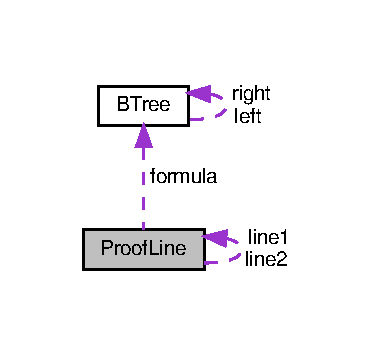
\includegraphics[width=180pt]{classProofLine__coll__graph}
\end{center}
\end{figure}
\subsection*{Public Member Functions}
\begin{DoxyCompactItemize}
\item 
\mbox{\hyperlink{classProofLine_a917582971a502aa8fc114467185c08b8}{Proof\+Line}} (int \mbox{\hyperlink{classProofLine_af1e2b73ad5275235028a4b131e574aa7}{line\+\_\+num}}, std\+::vector$<$ std\+::string $>$ parts, std\+::vector$<$ \mbox{\hyperlink{classProofLine}{Proof\+Line}} $\ast$$>$ prev\+\_\+lines)
\begin{DoxyCompactList}\small\item\em A constructor of \mbox{\hyperlink{classProofLine}{Proof\+Line}} for given inputs. \end{DoxyCompactList}\end{DoxyCompactItemize}
\subsection*{Public Attributes}
\begin{DoxyCompactItemize}
\item 
int \mbox{\hyperlink{classProofLine_af1e2b73ad5275235028a4b131e574aa7}{line\+\_\+num}}
\begin{DoxyCompactList}\small\item\em Line number of current \mbox{\hyperlink{classProofLine}{Proof\+Line}}. \end{DoxyCompactList}\item 
\mbox{\hyperlink{classBTree}{B\+Tree}} $\ast$ \mbox{\hyperlink{classProofLine_ac9dee0241ef4f6371135098fd5b1a66d}{formula}}
\begin{DoxyCompactList}\small\item\em Root of binary tree created from expression in input string. \end{DoxyCompactList}\item 
std\+::string \mbox{\hyperlink{classProofLine_acdc39e9e092a10ba3a6124f21c0eb420}{rule\+\_\+literal}}
\begin{DoxyCompactList}\small\item\em String of rule inputted. \end{DoxyCompactList}\item 
\mbox{\hyperlink{classProofLine}{Proof\+Line}} $\ast$ \mbox{\hyperlink{classProofLine_a7dbdcf0ea65aed377c5ac03303b474a6}{line1}}
\begin{DoxyCompactList}\small\item\em Pointer to \mbox{\hyperlink{classProofLine}{Proof\+Line}} with given line\+\_\+num. \end{DoxyCompactList}\item 
\mbox{\hyperlink{classProofLine}{Proof\+Line}} $\ast$ \mbox{\hyperlink{classProofLine_afed6bbbe21b20cdbde9398eb73ccf15f}{line2}}
\begin{DoxyCompactList}\small\item\em Pointer to \mbox{\hyperlink{classProofLine}{Proof\+Line}} with given line\+\_\+num. \end{DoxyCompactList}\item 
bool \mbox{\hyperlink{classProofLine_a8531e674967263c2e6ba67d8bf12a336}{is\+\_\+valid\+\_\+formula}}
\begin{DoxyCompactList}\small\item\em Whether current \mbox{\hyperlink{classProofLine}{Proof\+Line}} is true or false. \end{DoxyCompactList}\end{DoxyCompactItemize}
\subsection*{Related Functions}
(Note that these are not member functions.) \begin{DoxyCompactItemize}
\item 
bool \mbox{\hyperlink{classProofLine_ad34f3b0deb1e94d6b1c44a2de9680972}{check\+\_\+validity}} (\mbox{\hyperlink{classProofLine}{Proof\+Line}} $\ast$newline)
\begin{DoxyCompactList}\small\item\em Checks validity of given \mbox{\hyperlink{classProofLine}{Proof\+Line}}. \end{DoxyCompactList}\item 
bool \mbox{\hyperlink{classProofLine_a3d9c86a35ee3da94e663c41d40ff279b}{check\+\_\+valid\+\_\+prem}} (\mbox{\hyperlink{classProofLine}{Proof\+Line}} $\ast$newline)
\begin{DoxyCompactList}\small\item\em Checks validity of given P\+R\+E\+M\+I\+SE \mbox{\hyperlink{classProofLine}{Proof\+Line}}. \end{DoxyCompactList}\item 
bool \mbox{\hyperlink{classProofLine_a118aab7800af68c5b32fa5e103c75741}{check\+\_\+valid\+\_\+and\+\_\+i}} (\mbox{\hyperlink{classProofLine}{Proof\+Line}} $\ast$newline)
\begin{DoxyCompactList}\small\item\em Checks validity of given A\+ND I\+N\+T\+R\+O\+D\+U\+C\+T\+I\+ON \mbox{\hyperlink{classProofLine}{Proof\+Line}}. \end{DoxyCompactList}\item 
bool \mbox{\hyperlink{classProofLine_abdc10668ade35c80f0fd187c837e1a77}{check\+\_\+valid\+\_\+and\+\_\+e1}} (\mbox{\hyperlink{classProofLine}{Proof\+Line}} $\ast$newline)
\begin{DoxyCompactList}\small\item\em Checks validity of given A\+ND E\+L\+I\+M\+I\+N\+A\+T\+I\+ON 1 \mbox{\hyperlink{classProofLine}{Proof\+Line}}. \end{DoxyCompactList}\item 
bool \mbox{\hyperlink{classProofLine_add6d4592664b8ce7ed7e02f8f76a9a2a}{check\+\_\+valid\+\_\+and\+\_\+e2}} (\mbox{\hyperlink{classProofLine}{Proof\+Line}} $\ast$newline)
\begin{DoxyCompactList}\small\item\em Checks validity of given A\+ND E\+L\+I\+M\+I\+N\+A\+T\+I\+ON 2 \mbox{\hyperlink{classProofLine}{Proof\+Line}}. \end{DoxyCompactList}\item 
bool \mbox{\hyperlink{classProofLine_a2a3a60e30b9b569cacc3e2f1ec08747a}{check\+\_\+valid\+\_\+or\+\_\+i1}} (\mbox{\hyperlink{classProofLine}{Proof\+Line}} $\ast$newline)
\begin{DoxyCompactList}\small\item\em Checks validity of given OR I\+N\+T\+R\+O\+D\+U\+C\+T\+I\+ON 1 \mbox{\hyperlink{classProofLine}{Proof\+Line}}. \end{DoxyCompactList}\item 
bool \mbox{\hyperlink{classProofLine_abe95433e64d9bc565b87ccd6161a5db9}{check\+\_\+valid\+\_\+or\+\_\+i2}} (\mbox{\hyperlink{classProofLine}{Proof\+Line}} $\ast$newline)
\begin{DoxyCompactList}\small\item\em Checks validity of given OR I\+N\+T\+R\+O\+D\+U\+C\+T\+I\+ON 2 \mbox{\hyperlink{classProofLine}{Proof\+Line}}. \end{DoxyCompactList}\item 
bool \mbox{\hyperlink{classProofLine_a0c6ca18751b18ba87a745683438fe31a}{check\+\_\+valid\+\_\+impl\+\_\+e}} (\mbox{\hyperlink{classProofLine}{Proof\+Line}} $\ast$newline)
\begin{DoxyCompactList}\small\item\em Checks validity of given I\+M\+P\+L\+I\+C\+A\+T\+I\+ON E\+L\+I\+M\+I\+N\+A\+T\+I\+ON \mbox{\hyperlink{classProofLine}{Proof\+Line}}. \end{DoxyCompactList}\item 
bool \mbox{\hyperlink{classProofLine_a067d8de671da3f3ce43054723e31d232}{check\+\_\+valid\+\_\+mt}} (\mbox{\hyperlink{classProofLine}{Proof\+Line}} $\ast$newline)
\begin{DoxyCompactList}\small\item\em Checks validity of given M\+O\+D\+US T\+O\+L\+L\+E\+NS \mbox{\hyperlink{classProofLine}{Proof\+Line}}. \end{DoxyCompactList}\item 
\mbox{\hyperlink{classProofLine}{Proof\+Line}} $\ast$ \mbox{\hyperlink{classProofLine_ab2fe671562f60c3554c37ad75985e036}{parse\+\_\+line}} (std\+::string s, int \mbox{\hyperlink{classProofLine_af1e2b73ad5275235028a4b131e574aa7}{line\+\_\+num}}, std\+::vector$<$ \mbox{\hyperlink{classProofLine}{Proof\+Line}} $\ast$ $>$ prev\+\_\+lines)
\begin{DoxyCompactList}\small\item\em Makes new \mbox{\hyperlink{classProofLine}{Proof\+Line}} object using the input string. \end{DoxyCompactList}\item 
void \mbox{\hyperlink{classProofLine_a43022f1f1f94d244fad4a528ef0a8726}{validate\+\_\+proof}} ()
\begin{DoxyCompactList}\small\item\em Checks validity of user-\/given proof. \end{DoxyCompactList}\end{DoxyCompactItemize}


\subsection{Detailed Description}
Class containing segregated information about a \mbox{\hyperlink{classProofLine}{Proof\+Line}}. 

\subsection{Constructor \& Destructor Documentation}
\mbox{\Hypertarget{classProofLine_a917582971a502aa8fc114467185c08b8}\label{classProofLine_a917582971a502aa8fc114467185c08b8}} 
\index{Proof\+Line@{Proof\+Line}!Proof\+Line@{Proof\+Line}}
\index{Proof\+Line@{Proof\+Line}!Proof\+Line@{Proof\+Line}}
\subsubsection{\texorpdfstring{Proof\+Line()}{ProofLine()}}
{\footnotesize\ttfamily Proof\+Line\+::\+Proof\+Line (\begin{DoxyParamCaption}\item[{int}]{line\+\_\+num,  }\item[{std\+::vector$<$ std\+::string $>$}]{parts,  }\item[{std\+::vector$<$ \mbox{\hyperlink{classProofLine}{Proof\+Line}} $\ast$$>$}]{prev\+\_\+lines }\end{DoxyParamCaption})}



A constructor of \mbox{\hyperlink{classProofLine}{Proof\+Line}} for given inputs. 


\begin{DoxyParams}[1]{Parameters}
\mbox{\texttt{ in}}  & {\em line\+\_\+num} & Line number of current \mbox{\hyperlink{classProofLine}{Proof\+Line}} \\
\hline
\mbox{\texttt{ in}}  & {\em parts} & Vector of strings created by splitting of input string with delimiter \textquotesingle{}/\textquotesingle{} \\
\hline
\mbox{\texttt{ in}}  & {\em prev\+\_\+lines} & Vector of pointers to all previous \mbox{\hyperlink{classProofLine}{Proof\+Line}} \\
\hline
\end{DoxyParams}


\subsection{Friends And Related Function Documentation}
\mbox{\Hypertarget{classProofLine_ad34f3b0deb1e94d6b1c44a2de9680972}\label{classProofLine_ad34f3b0deb1e94d6b1c44a2de9680972}} 
\index{Proof\+Line@{Proof\+Line}!check\+\_\+validity@{check\+\_\+validity}}
\index{check\+\_\+validity@{check\+\_\+validity}!Proof\+Line@{Proof\+Line}}
\subsubsection{\texorpdfstring{check\+\_\+validity()}{check\_validity()}}
{\footnotesize\ttfamily bool check\+\_\+validity (\begin{DoxyParamCaption}\item[{\mbox{\hyperlink{classProofLine}{Proof\+Line}} $\ast$}]{newline }\end{DoxyParamCaption})\hspace{0.3cm}{\ttfamily [related]}}



Checks validity of given \mbox{\hyperlink{classProofLine}{Proof\+Line}}. 

Complexity\+: O(1) 
\begin{DoxyParams}[1]{Parameters}
\mbox{\texttt{ in}}  & {\em newline} & Pointer to \mbox{\hyperlink{classProofLine}{Proof\+Line}} to be validated \\
\hline
\end{DoxyParams}
\begin{DoxyReturn}{Returns}
true if the \mbox{\hyperlink{classProofLine}{Proof\+Line}} is valid else false 
\end{DoxyReturn}
\mbox{\Hypertarget{classProofLine_a3d9c86a35ee3da94e663c41d40ff279b}\label{classProofLine_a3d9c86a35ee3da94e663c41d40ff279b}} 
\index{Proof\+Line@{Proof\+Line}!check\+\_\+valid\+\_\+prem@{check\+\_\+valid\+\_\+prem}}
\index{check\+\_\+valid\+\_\+prem@{check\+\_\+valid\+\_\+prem}!Proof\+Line@{Proof\+Line}}
\subsubsection{\texorpdfstring{check\+\_\+valid\+\_\+prem()}{check\_valid\_prem()}}
{\footnotesize\ttfamily bool check\+\_\+valid\+\_\+prem (\begin{DoxyParamCaption}\item[{\mbox{\hyperlink{classProofLine}{Proof\+Line}} $\ast$}]{newline }\end{DoxyParamCaption})\hspace{0.3cm}{\ttfamily [related]}}



Checks validity of given P\+R\+E\+M\+I\+SE \mbox{\hyperlink{classProofLine}{Proof\+Line}}. 

Complexity\+: O(1) 
\begin{DoxyParams}[1]{Parameters}
\mbox{\texttt{ in}}  & {\em newline} & Pointer to the P\+R\+E\+M\+I\+SE \mbox{\hyperlink{classProofLine}{Proof\+Line}} \\
\hline
\end{DoxyParams}
\begin{DoxyReturn}{Returns}
true if \mbox{\hyperlink{classProofLine}{Proof\+Line}} is a P\+R\+E\+M\+I\+SE else false 
\end{DoxyReturn}
\mbox{\Hypertarget{classProofLine_a118aab7800af68c5b32fa5e103c75741}\label{classProofLine_a118aab7800af68c5b32fa5e103c75741}} 
\index{Proof\+Line@{Proof\+Line}!check\+\_\+valid\+\_\+and\+\_\+i@{check\+\_\+valid\+\_\+and\+\_\+i}}
\index{check\+\_\+valid\+\_\+and\+\_\+i@{check\+\_\+valid\+\_\+and\+\_\+i}!Proof\+Line@{Proof\+Line}}
\subsubsection{\texorpdfstring{check\+\_\+valid\+\_\+and\+\_\+i()}{check\_valid\_and\_i()}}
{\footnotesize\ttfamily bool check\+\_\+valid\+\_\+and\+\_\+i (\begin{DoxyParamCaption}\item[{\mbox{\hyperlink{classProofLine}{Proof\+Line}} $\ast$}]{newline }\end{DoxyParamCaption})\hspace{0.3cm}{\ttfamily [related]}}



Checks validity of given A\+ND I\+N\+T\+R\+O\+D\+U\+C\+T\+I\+ON \mbox{\hyperlink{classProofLine}{Proof\+Line}}. 

Complexity\+: O(1) 
\begin{DoxyParams}[1]{Parameters}
\mbox{\texttt{ in}}  & {\em newline} & Pointer to the A\+ND I\+N\+T\+R\+O\+D\+U\+C\+T\+I\+ON \mbox{\hyperlink{classProofLine}{Proof\+Line}} \\
\hline
\end{DoxyParams}
\begin{DoxyReturn}{Returns}
true if the \mbox{\hyperlink{classProofLine}{Proof\+Line}} is valid else false 
\end{DoxyReturn}
\mbox{\Hypertarget{classProofLine_abdc10668ade35c80f0fd187c837e1a77}\label{classProofLine_abdc10668ade35c80f0fd187c837e1a77}} 
\index{Proof\+Line@{Proof\+Line}!check\+\_\+valid\+\_\+and\+\_\+e1@{check\+\_\+valid\+\_\+and\+\_\+e1}}
\index{check\+\_\+valid\+\_\+and\+\_\+e1@{check\+\_\+valid\+\_\+and\+\_\+e1}!Proof\+Line@{Proof\+Line}}
\subsubsection{\texorpdfstring{check\+\_\+valid\+\_\+and\+\_\+e1()}{check\_valid\_and\_e1()}}
{\footnotesize\ttfamily bool check\+\_\+valid\+\_\+and\+\_\+e1 (\begin{DoxyParamCaption}\item[{\mbox{\hyperlink{classProofLine}{Proof\+Line}} $\ast$}]{newline }\end{DoxyParamCaption})\hspace{0.3cm}{\ttfamily [related]}}



Checks validity of given A\+ND E\+L\+I\+M\+I\+N\+A\+T\+I\+ON 1 \mbox{\hyperlink{classProofLine}{Proof\+Line}}. 

Complexity\+: O(1) 
\begin{DoxyParams}[1]{Parameters}
\mbox{\texttt{ in}}  & {\em newline} & Pointer to the A\+ND E\+L\+I\+M\+I\+N\+A\+T\+I\+ON 1 \mbox{\hyperlink{classProofLine}{Proof\+Line}} \\
\hline
\end{DoxyParams}
\begin{DoxyReturn}{Returns}
true if the \mbox{\hyperlink{classProofLine}{Proof\+Line}} is valid else false 
\end{DoxyReturn}
\mbox{\Hypertarget{classProofLine_add6d4592664b8ce7ed7e02f8f76a9a2a}\label{classProofLine_add6d4592664b8ce7ed7e02f8f76a9a2a}} 
\index{Proof\+Line@{Proof\+Line}!check\+\_\+valid\+\_\+and\+\_\+e2@{check\+\_\+valid\+\_\+and\+\_\+e2}}
\index{check\+\_\+valid\+\_\+and\+\_\+e2@{check\+\_\+valid\+\_\+and\+\_\+e2}!Proof\+Line@{Proof\+Line}}
\subsubsection{\texorpdfstring{check\+\_\+valid\+\_\+and\+\_\+e2()}{check\_valid\_and\_e2()}}
{\footnotesize\ttfamily bool check\+\_\+valid\+\_\+and\+\_\+e2 (\begin{DoxyParamCaption}\item[{\mbox{\hyperlink{classProofLine}{Proof\+Line}} $\ast$}]{newline }\end{DoxyParamCaption})\hspace{0.3cm}{\ttfamily [related]}}



Checks validity of given A\+ND E\+L\+I\+M\+I\+N\+A\+T\+I\+ON 2 \mbox{\hyperlink{classProofLine}{Proof\+Line}}. 

Complexity\+: O(1) 
\begin{DoxyParams}[1]{Parameters}
\mbox{\texttt{ in}}  & {\em newline} & Pointer to the A\+ND E\+L\+I\+M\+I\+N\+A\+T\+I\+ON 2 \mbox{\hyperlink{classProofLine}{Proof\+Line}} \\
\hline
\end{DoxyParams}
\begin{DoxyReturn}{Returns}
true if the \mbox{\hyperlink{classProofLine}{Proof\+Line}} is valid else false 
\end{DoxyReturn}
\mbox{\Hypertarget{classProofLine_a2a3a60e30b9b569cacc3e2f1ec08747a}\label{classProofLine_a2a3a60e30b9b569cacc3e2f1ec08747a}} 
\index{Proof\+Line@{Proof\+Line}!check\+\_\+valid\+\_\+or\+\_\+i1@{check\+\_\+valid\+\_\+or\+\_\+i1}}
\index{check\+\_\+valid\+\_\+or\+\_\+i1@{check\+\_\+valid\+\_\+or\+\_\+i1}!Proof\+Line@{Proof\+Line}}
\subsubsection{\texorpdfstring{check\+\_\+valid\+\_\+or\+\_\+i1()}{check\_valid\_or\_i1()}}
{\footnotesize\ttfamily bool check\+\_\+valid\+\_\+or\+\_\+i1 (\begin{DoxyParamCaption}\item[{\mbox{\hyperlink{classProofLine}{Proof\+Line}} $\ast$}]{newline }\end{DoxyParamCaption})\hspace{0.3cm}{\ttfamily [related]}}



Checks validity of given OR I\+N\+T\+R\+O\+D\+U\+C\+T\+I\+ON 1 \mbox{\hyperlink{classProofLine}{Proof\+Line}}. 

Complexity\+: O(1) 
\begin{DoxyParams}[1]{Parameters}
\mbox{\texttt{ in}}  & {\em newline} & Pointer to the OR I\+N\+T\+R\+O\+D\+U\+C\+T\+I\+ON 1 \mbox{\hyperlink{classProofLine}{Proof\+Line}} \\
\hline
\end{DoxyParams}
\begin{DoxyReturn}{Returns}
true if the \mbox{\hyperlink{classProofLine}{Proof\+Line}} is valid else false 
\end{DoxyReturn}
\mbox{\Hypertarget{classProofLine_abe95433e64d9bc565b87ccd6161a5db9}\label{classProofLine_abe95433e64d9bc565b87ccd6161a5db9}} 
\index{Proof\+Line@{Proof\+Line}!check\+\_\+valid\+\_\+or\+\_\+i2@{check\+\_\+valid\+\_\+or\+\_\+i2}}
\index{check\+\_\+valid\+\_\+or\+\_\+i2@{check\+\_\+valid\+\_\+or\+\_\+i2}!Proof\+Line@{Proof\+Line}}
\subsubsection{\texorpdfstring{check\+\_\+valid\+\_\+or\+\_\+i2()}{check\_valid\_or\_i2()}}
{\footnotesize\ttfamily bool check\+\_\+valid\+\_\+or\+\_\+i2 (\begin{DoxyParamCaption}\item[{\mbox{\hyperlink{classProofLine}{Proof\+Line}} $\ast$}]{newline }\end{DoxyParamCaption})\hspace{0.3cm}{\ttfamily [related]}}



Checks validity of given OR I\+N\+T\+R\+O\+D\+U\+C\+T\+I\+ON 2 \mbox{\hyperlink{classProofLine}{Proof\+Line}}. 

Complexity\+: O(1) 
\begin{DoxyParams}[1]{Parameters}
\mbox{\texttt{ in}}  & {\em newline} & Pointer to the OR I\+N\+T\+R\+O\+D\+U\+C\+T\+I\+ON 2 \mbox{\hyperlink{classProofLine}{Proof\+Line}} \\
\hline
\end{DoxyParams}
\begin{DoxyReturn}{Returns}
true if the \mbox{\hyperlink{classProofLine}{Proof\+Line}} is valid else false 
\end{DoxyReturn}
\mbox{\Hypertarget{classProofLine_a0c6ca18751b18ba87a745683438fe31a}\label{classProofLine_a0c6ca18751b18ba87a745683438fe31a}} 
\index{Proof\+Line@{Proof\+Line}!check\+\_\+valid\+\_\+impl\+\_\+e@{check\+\_\+valid\+\_\+impl\+\_\+e}}
\index{check\+\_\+valid\+\_\+impl\+\_\+e@{check\+\_\+valid\+\_\+impl\+\_\+e}!Proof\+Line@{Proof\+Line}}
\subsubsection{\texorpdfstring{check\+\_\+valid\+\_\+impl\+\_\+e()}{check\_valid\_impl\_e()}}
{\footnotesize\ttfamily bool check\+\_\+valid\+\_\+impl\+\_\+e (\begin{DoxyParamCaption}\item[{\mbox{\hyperlink{classProofLine}{Proof\+Line}} $\ast$}]{newline }\end{DoxyParamCaption})\hspace{0.3cm}{\ttfamily [related]}}



Checks validity of given I\+M\+P\+L\+I\+C\+A\+T\+I\+ON E\+L\+I\+M\+I\+N\+A\+T\+I\+ON \mbox{\hyperlink{classProofLine}{Proof\+Line}}. 

Complexity\+: O(1) 
\begin{DoxyParams}[1]{Parameters}
\mbox{\texttt{ in}}  & {\em newline} & Pointer to the I\+M\+P\+L\+I\+C\+A\+T\+I\+ON E\+L\+I\+M\+I\+N\+A\+T\+I\+ON \mbox{\hyperlink{classProofLine}{Proof\+Line}} \\
\hline
\end{DoxyParams}
\begin{DoxyReturn}{Returns}
true if the \mbox{\hyperlink{classProofLine}{Proof\+Line}} is valid else false 
\end{DoxyReturn}
\mbox{\Hypertarget{classProofLine_a067d8de671da3f3ce43054723e31d232}\label{classProofLine_a067d8de671da3f3ce43054723e31d232}} 
\index{Proof\+Line@{Proof\+Line}!check\+\_\+valid\+\_\+mt@{check\+\_\+valid\+\_\+mt}}
\index{check\+\_\+valid\+\_\+mt@{check\+\_\+valid\+\_\+mt}!Proof\+Line@{Proof\+Line}}
\subsubsection{\texorpdfstring{check\+\_\+valid\+\_\+mt()}{check\_valid\_mt()}}
{\footnotesize\ttfamily bool check\+\_\+valid\+\_\+mt (\begin{DoxyParamCaption}\item[{\mbox{\hyperlink{classProofLine}{Proof\+Line}} $\ast$}]{newline }\end{DoxyParamCaption})\hspace{0.3cm}{\ttfamily [related]}}



Checks validity of given M\+O\+D\+US T\+O\+L\+L\+E\+NS \mbox{\hyperlink{classProofLine}{Proof\+Line}}. 

Complexity\+: O(1) 
\begin{DoxyParams}[1]{Parameters}
\mbox{\texttt{ in}}  & {\em newline} & Pointer to the M\+O\+D\+US T\+O\+L\+L\+E\+NS \mbox{\hyperlink{classProofLine}{Proof\+Line}} \\
\hline
\end{DoxyParams}
\begin{DoxyReturn}{Returns}
true if the \mbox{\hyperlink{classProofLine}{Proof\+Line}} is valid else false 
\end{DoxyReturn}
\mbox{\Hypertarget{classProofLine_ab2fe671562f60c3554c37ad75985e036}\label{classProofLine_ab2fe671562f60c3554c37ad75985e036}} 
\index{Proof\+Line@{Proof\+Line}!parse\+\_\+line@{parse\+\_\+line}}
\index{parse\+\_\+line@{parse\+\_\+line}!Proof\+Line@{Proof\+Line}}
\subsubsection{\texorpdfstring{parse\+\_\+line()}{parse\_line()}}
{\footnotesize\ttfamily \mbox{\hyperlink{classProofLine}{Proof\+Line}} $\ast$ parse\+\_\+line (\begin{DoxyParamCaption}\item[{std\+::string}]{s,  }\item[{int}]{line\+\_\+num,  }\item[{std\+::vector$<$ \mbox{\hyperlink{classProofLine}{Proof\+Line}} $\ast$ $>$}]{prev\+\_\+lines }\end{DoxyParamCaption})\hspace{0.3cm}{\ttfamily [related]}}



Makes new \mbox{\hyperlink{classProofLine}{Proof\+Line}} object using the input string. 


\begin{DoxyParams}[1]{Parameters}
\mbox{\texttt{ in}}  & {\em s} & Input string obtained from user \\
\hline
\mbox{\texttt{ in}}  & {\em line\+\_\+num} & Line number of current \mbox{\hyperlink{classProofLine}{Proof\+Line}} \\
\hline
\mbox{\texttt{ in}}  & {\em prev\+\_\+lines} & Vector containing all previous \mbox{\hyperlink{classProofLine}{Proof\+Line}} pointers \\
\hline
\end{DoxyParams}
\begin{DoxyReturn}{Returns}
Pointer to newly created \mbox{\hyperlink{classProofLine}{Proof\+Line}} object 
\end{DoxyReturn}
\mbox{\Hypertarget{classProofLine_a43022f1f1f94d244fad4a528ef0a8726}\label{classProofLine_a43022f1f1f94d244fad4a528ef0a8726}} 
\index{Proof\+Line@{Proof\+Line}!validate\+\_\+proof@{validate\+\_\+proof}}
\index{validate\+\_\+proof@{validate\+\_\+proof}!Proof\+Line@{Proof\+Line}}
\subsubsection{\texorpdfstring{validate\+\_\+proof()}{validate\_proof()}}
{\footnotesize\ttfamily void validate\+\_\+proof (\begin{DoxyParamCaption}{ }\end{DoxyParamCaption})\hspace{0.3cm}{\ttfamily [related]}}



Checks validity of user-\/given proof. 



\subsection{Member Data Documentation}
\mbox{\Hypertarget{classProofLine_af1e2b73ad5275235028a4b131e574aa7}\label{classProofLine_af1e2b73ad5275235028a4b131e574aa7}} 
\index{Proof\+Line@{Proof\+Line}!line\+\_\+num@{line\+\_\+num}}
\index{line\+\_\+num@{line\+\_\+num}!Proof\+Line@{Proof\+Line}}
\subsubsection{\texorpdfstring{line\+\_\+num}{line\_num}}
{\footnotesize\ttfamily int Proof\+Line\+::line\+\_\+num}



Line number of current \mbox{\hyperlink{classProofLine}{Proof\+Line}}. 

\mbox{\Hypertarget{classProofLine_ac9dee0241ef4f6371135098fd5b1a66d}\label{classProofLine_ac9dee0241ef4f6371135098fd5b1a66d}} 
\index{Proof\+Line@{Proof\+Line}!formula@{formula}}
\index{formula@{formula}!Proof\+Line@{Proof\+Line}}
\subsubsection{\texorpdfstring{formula}{formula}}
{\footnotesize\ttfamily \mbox{\hyperlink{classBTree}{B\+Tree}}$\ast$ Proof\+Line\+::formula}



Root of binary tree created from expression in input string. 

\mbox{\Hypertarget{classProofLine_acdc39e9e092a10ba3a6124f21c0eb420}\label{classProofLine_acdc39e9e092a10ba3a6124f21c0eb420}} 
\index{Proof\+Line@{Proof\+Line}!rule\+\_\+literal@{rule\+\_\+literal}}
\index{rule\+\_\+literal@{rule\+\_\+literal}!Proof\+Line@{Proof\+Line}}
\subsubsection{\texorpdfstring{rule\+\_\+literal}{rule\_literal}}
{\footnotesize\ttfamily std\+::string Proof\+Line\+::rule\+\_\+literal}



String of rule inputted. 

\mbox{\Hypertarget{classProofLine_a7dbdcf0ea65aed377c5ac03303b474a6}\label{classProofLine_a7dbdcf0ea65aed377c5ac03303b474a6}} 
\index{Proof\+Line@{Proof\+Line}!line1@{line1}}
\index{line1@{line1}!Proof\+Line@{Proof\+Line}}
\subsubsection{\texorpdfstring{line1}{line1}}
{\footnotesize\ttfamily \mbox{\hyperlink{classProofLine}{Proof\+Line}}$\ast$ Proof\+Line\+::line1}



Pointer to \mbox{\hyperlink{classProofLine}{Proof\+Line}} with given line\+\_\+num. 

\mbox{\Hypertarget{classProofLine_afed6bbbe21b20cdbde9398eb73ccf15f}\label{classProofLine_afed6bbbe21b20cdbde9398eb73ccf15f}} 
\index{Proof\+Line@{Proof\+Line}!line2@{line2}}
\index{line2@{line2}!Proof\+Line@{Proof\+Line}}
\subsubsection{\texorpdfstring{line2}{line2}}
{\footnotesize\ttfamily \mbox{\hyperlink{classProofLine}{Proof\+Line}}$\ast$ Proof\+Line\+::line2}



Pointer to \mbox{\hyperlink{classProofLine}{Proof\+Line}} with given line\+\_\+num. 

\mbox{\Hypertarget{classProofLine_a8531e674967263c2e6ba67d8bf12a336}\label{classProofLine_a8531e674967263c2e6ba67d8bf12a336}} 
\index{Proof\+Line@{Proof\+Line}!is\+\_\+valid\+\_\+formula@{is\+\_\+valid\+\_\+formula}}
\index{is\+\_\+valid\+\_\+formula@{is\+\_\+valid\+\_\+formula}!Proof\+Line@{Proof\+Line}}
\subsubsection{\texorpdfstring{is\+\_\+valid\+\_\+formula}{is\_valid\_formula}}
{\footnotesize\ttfamily bool Proof\+Line\+::is\+\_\+valid\+\_\+formula}



Whether current \mbox{\hyperlink{classProofLine}{Proof\+Line}} is true or false. 



The documentation for this class was generated from the following files\+:\begin{DoxyCompactItemize}
\item 
\mbox{\hyperlink{task2_8h}{task2.\+h}}\item 
\mbox{\hyperlink{rules_8h}{rules.\+h}}\item 
\mbox{\hyperlink{task2_8cpp}{task2.\+cpp}}\end{DoxyCompactItemize}

\chapter{File Documentation}
\hypertarget{BTree_8cpp}{}\section{B\+Tree.\+cpp File Reference}
\label{BTree_8cpp}\index{B\+Tree.\+cpp@{B\+Tree.\+cpp}}
{\ttfamily \#include \char`\"{}B\+Tree.\+h\char`\"{}}\newline
Include dependency graph for B\+Tree.\+cpp\+:

\hypertarget{BTree_8h}{}\section{B\+Tree.\+h File Reference}
\label{BTree_8h}\index{B\+Tree.\+h@{B\+Tree.\+h}}
{\ttfamily \#include $<$string$>$}\newline
Include dependency graph for B\+Tree.\+h\+:
% FIG 0
This graph shows which files directly or indirectly include this file\+:
% FIG 1
\subsection*{Classes}
\begin{DoxyCompactItemize}
\item 
class \hyperlink{classBTree}{B\+Tree}
\end{DoxyCompactItemize}

\hypertarget{main_8cpp}{}\section{main.\+cpp File Reference}
\label{main_8cpp}\index{main.\+cpp@{main.\+cpp}}
{\ttfamily \#include $<$iostream$>$}\newline
{\ttfamily \#include \char`\"{}task1.\+h\char`\"{}}\newline
{\ttfamily \#include \char`\"{}task2.\+h\char`\"{}}\newline
Include dependency graph for main.\+cpp\+:\nopagebreak
\begin{figure}[H]
\begin{center}
\leavevmode
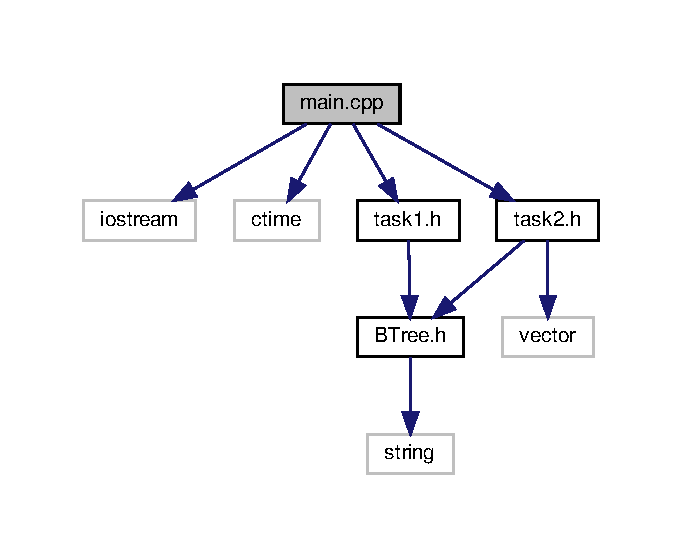
\includegraphics[width=269pt]{main_8cpp__incl}
\end{center}
\end{figure}
\subsection*{Functions}
\begin{DoxyCompactItemize}
\item 
int \mbox{\hyperlink{main_8cpp_ae66f6b31b5ad750f1fe042a706a4e3d4}{main}} ()
\end{DoxyCompactItemize}


\subsection{Function Documentation}
\mbox{\Hypertarget{main_8cpp_ae66f6b31b5ad750f1fe042a706a4e3d4}\label{main_8cpp_ae66f6b31b5ad750f1fe042a706a4e3d4}} 
\index{main.\+cpp@{main.\+cpp}!main@{main}}
\index{main@{main}!main.\+cpp@{main.\+cpp}}
\subsubsection{\texorpdfstring{main()}{main()}}
{\footnotesize\ttfamily int main (\begin{DoxyParamCaption}{ }\end{DoxyParamCaption})}


\hypertarget{operators_8cpp}{}\section{operators.\+cpp File Reference}
\label{operators_8cpp}\index{operators.\+cpp@{operators.\+cpp}}
{\ttfamily \#include \char`\"{}operators.\+h\char`\"{}}\newline
Include dependency graph for operators.\+cpp\+:\nopagebreak
\begin{figure}[H]
\begin{center}
\leavevmode
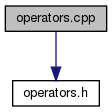
\includegraphics[width=156pt]{operators_8cpp__incl}
\end{center}
\end{figure}
\subsection*{Functions}
\begin{DoxyCompactItemize}
\item 
bool \mbox{\hyperlink{operators_8cpp_add6a2ed794331617fad3b9a2dee85aff}{is\+\_\+operand}} (char token)
\begin{DoxyCompactList}\small\item\em Checks whether token is an operand. \end{DoxyCompactList}\item 
bool \mbox{\hyperlink{operators_8cpp_a10228ed592f29bc85c70f7652ccc0510}{is\+\_\+operator}} (char token)
\begin{DoxyCompactList}\small\item\em Checks whether token is an operator. \end{DoxyCompactList}\item 
int \mbox{\hyperlink{operators_8cpp_a8a4ebbb3e294da2153247286fd741cd8}{op\+\_\+priority}} (char op)
\begin{DoxyCompactList}\small\item\em Assigns priority(precedence) to op. \end{DoxyCompactList}\end{DoxyCompactItemize}


\subsection{Function Documentation}
\mbox{\Hypertarget{operators_8cpp_add6a2ed794331617fad3b9a2dee85aff}\label{operators_8cpp_add6a2ed794331617fad3b9a2dee85aff}} 
\index{operators.\+cpp@{operators.\+cpp}!is\+\_\+operand@{is\+\_\+operand}}
\index{is\+\_\+operand@{is\+\_\+operand}!operators.\+cpp@{operators.\+cpp}}
\subsubsection{\texorpdfstring{is\+\_\+operand()}{is\_operand()}}
{\footnotesize\ttfamily bool is\+\_\+operand (\begin{DoxyParamCaption}\item[{char}]{token }\end{DoxyParamCaption})}



Checks whether token is an operand. 

Complexity\+: O(1) 
\begin{DoxyParams}[1]{Parameters}
\mbox{\texttt{ in}}  & {\em token} & Character which is to be checked \\
\hline
\end{DoxyParams}
\begin{DoxyReturn}{Returns}
true if token is an operand else false 
\end{DoxyReturn}
\mbox{\Hypertarget{operators_8cpp_a10228ed592f29bc85c70f7652ccc0510}\label{operators_8cpp_a10228ed592f29bc85c70f7652ccc0510}} 
\index{operators.\+cpp@{operators.\+cpp}!is\+\_\+operator@{is\+\_\+operator}}
\index{is\+\_\+operator@{is\+\_\+operator}!operators.\+cpp@{operators.\+cpp}}
\subsubsection{\texorpdfstring{is\+\_\+operator()}{is\_operator()}}
{\footnotesize\ttfamily bool is\+\_\+operator (\begin{DoxyParamCaption}\item[{char}]{token }\end{DoxyParamCaption})}



Checks whether token is an operator. 

Complexity\+: O(number of valid operators) 
\begin{DoxyParams}[1]{Parameters}
\mbox{\texttt{ in}}  & {\em token} & Character which is to be checked \\
\hline
\end{DoxyParams}
\begin{DoxyReturn}{Returns}
true if token is an operator else false 
\end{DoxyReturn}
\mbox{\Hypertarget{operators_8cpp_a8a4ebbb3e294da2153247286fd741cd8}\label{operators_8cpp_a8a4ebbb3e294da2153247286fd741cd8}} 
\index{operators.\+cpp@{operators.\+cpp}!op\+\_\+priority@{op\+\_\+priority}}
\index{op\+\_\+priority@{op\+\_\+priority}!operators.\+cpp@{operators.\+cpp}}
\subsubsection{\texorpdfstring{op\+\_\+priority()}{op\_priority()}}
{\footnotesize\ttfamily int op\+\_\+priority (\begin{DoxyParamCaption}\item[{char}]{op }\end{DoxyParamCaption})}



Assigns priority(precedence) to op. 

Assigns integer priority using the following order\+: N\+E\+G(4) $>$ A\+N\+D(3) = O\+R(3) $>$ I\+M\+P\+L(2) with default being -\/1~\newline
 Complexity\+: O(1) 
\begin{DoxyParams}[1]{Parameters}
\mbox{\texttt{ in}}  & {\em op} & Character whose priority is to be determined \\
\hline
\end{DoxyParams}
\begin{DoxyReturn}{Returns}
Corresponding priority integer 
\end{DoxyReturn}

\hypertarget{operators_8h}{}\section{operators.\+h File Reference}
\label{operators_8h}\index{operators.\+h@{operators.\+h}}
This graph shows which files directly or indirectly include this file\+:\nopagebreak
\begin{figure}[H]
\begin{center}
\leavevmode
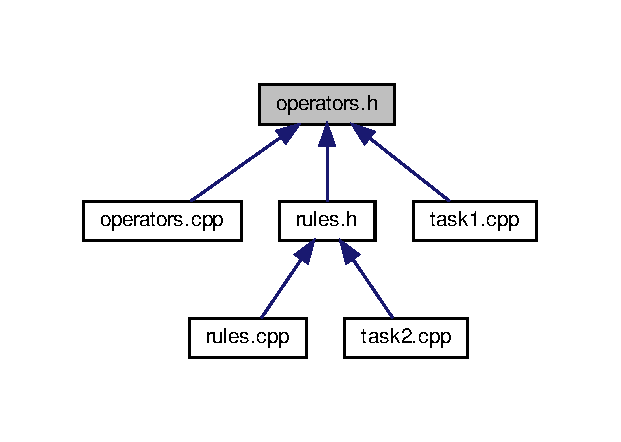
\includegraphics[width=298pt]{operators_8h__dep__incl}
\end{center}
\end{figure}
\subsection*{Namespaces}
\begin{DoxyCompactItemize}
\item 
 \mbox{\hyperlink{namespaceoperators}{operators}}
\begin{DoxyCompactList}\small\item\em Defining operators using namespace to make it easy for changing input syntax as and when required. \end{DoxyCompactList}\end{DoxyCompactItemize}
\subsection*{Functions}
\begin{DoxyCompactItemize}
\item 
bool \mbox{\hyperlink{operators_8h_add6a2ed794331617fad3b9a2dee85aff}{is\+\_\+operand}} (char token)
\begin{DoxyCompactList}\small\item\em Checks whether token is an operand. \end{DoxyCompactList}\item 
bool \mbox{\hyperlink{operators_8h_a10228ed592f29bc85c70f7652ccc0510}{is\+\_\+operator}} (char token)
\begin{DoxyCompactList}\small\item\em Checks whether token is an operator. \end{DoxyCompactList}\item 
int \mbox{\hyperlink{operators_8h_a8a4ebbb3e294da2153247286fd741cd8}{op\+\_\+priority}} (char op)
\begin{DoxyCompactList}\small\item\em Assigns priority(precedence) to op. \end{DoxyCompactList}\end{DoxyCompactItemize}
\subsection*{Variables}
\begin{DoxyCompactItemize}
\item 
const char \mbox{\hyperlink{namespaceoperators_abc0d09c09b437de98007962a590ea557}{operators\+::\+N\+EG}} \{\textquotesingle{}$\sim$\textquotesingle{}\}
\begin{DoxyCompactList}\small\item\em Defines N\+E\+G\+A\+T\+I\+ON. \end{DoxyCompactList}\item 
const char \mbox{\hyperlink{namespaceoperators_aff9dc11d489d31278c1e3f90ae09dd9b}{operators\+::\+A\+ND}} \{\textquotesingle{}$^\wedge$\textquotesingle{}\}
\begin{DoxyCompactList}\small\item\em Defines A\+ND. \end{DoxyCompactList}\item 
const char \mbox{\hyperlink{namespaceoperators_a1f469207e0d08770fc7bbac128cfd845}{operators\+::\+OR}} \{\textquotesingle{}V\textquotesingle{}\}
\begin{DoxyCompactList}\small\item\em Defines OR. \end{DoxyCompactList}\item 
const char \mbox{\hyperlink{namespaceoperators_a40fe490f326324304d4529854fb2deea}{operators\+::\+I\+M\+PL}} \{\textquotesingle{}$>$\textquotesingle{}\}
\begin{DoxyCompactList}\small\item\em Defines I\+M\+P\+L\+I\+C\+A\+T\+I\+ON. \end{DoxyCompactList}\end{DoxyCompactItemize}


\subsection{Function Documentation}
\mbox{\Hypertarget{operators_8h_add6a2ed794331617fad3b9a2dee85aff}\label{operators_8h_add6a2ed794331617fad3b9a2dee85aff}} 
\index{operators.\+h@{operators.\+h}!is\+\_\+operand@{is\+\_\+operand}}
\index{is\+\_\+operand@{is\+\_\+operand}!operators.\+h@{operators.\+h}}
\subsubsection{\texorpdfstring{is\+\_\+operand()}{is\_operand()}}
{\footnotesize\ttfamily bool is\+\_\+operand (\begin{DoxyParamCaption}\item[{char}]{token }\end{DoxyParamCaption})}



Checks whether token is an operand. 

Complexity\+: O(1) 
\begin{DoxyParams}[1]{Parameters}
\mbox{\texttt{ in}}  & {\em token} & Character which is to be checked \\
\hline
\end{DoxyParams}
\begin{DoxyReturn}{Returns}
true if token is an operand else false 
\end{DoxyReturn}
\mbox{\Hypertarget{operators_8h_a10228ed592f29bc85c70f7652ccc0510}\label{operators_8h_a10228ed592f29bc85c70f7652ccc0510}} 
\index{operators.\+h@{operators.\+h}!is\+\_\+operator@{is\+\_\+operator}}
\index{is\+\_\+operator@{is\+\_\+operator}!operators.\+h@{operators.\+h}}
\subsubsection{\texorpdfstring{is\+\_\+operator()}{is\_operator()}}
{\footnotesize\ttfamily bool is\+\_\+operator (\begin{DoxyParamCaption}\item[{char}]{token }\end{DoxyParamCaption})}



Checks whether token is an operator. 

Complexity\+: O(number of valid operators) 
\begin{DoxyParams}[1]{Parameters}
\mbox{\texttt{ in}}  & {\em token} & Character which is to be checked \\
\hline
\end{DoxyParams}
\begin{DoxyReturn}{Returns}
true if token is an operator else false 
\end{DoxyReturn}
\mbox{\Hypertarget{operators_8h_a8a4ebbb3e294da2153247286fd741cd8}\label{operators_8h_a8a4ebbb3e294da2153247286fd741cd8}} 
\index{operators.\+h@{operators.\+h}!op\+\_\+priority@{op\+\_\+priority}}
\index{op\+\_\+priority@{op\+\_\+priority}!operators.\+h@{operators.\+h}}
\subsubsection{\texorpdfstring{op\+\_\+priority()}{op\_priority()}}
{\footnotesize\ttfamily int op\+\_\+priority (\begin{DoxyParamCaption}\item[{char}]{op }\end{DoxyParamCaption})}



Assigns priority(precedence) to op. 

Assigns integer priority using the following order\+: N\+E\+G(4) $>$ A\+N\+D(3) = O\+R(3) $>$ I\+M\+P\+L(2) with default being -\/1~\newline
 Complexity\+: O(1) 
\begin{DoxyParams}[1]{Parameters}
\mbox{\texttt{ in}}  & {\em op} & Character whose priority is to be determined \\
\hline
\end{DoxyParams}
\begin{DoxyReturn}{Returns}
Corresponding priority integer 
\end{DoxyReturn}

\hypertarget{README_8md}{}\section{R\+E\+A\+D\+M\+E.\+md File Reference}
\label{README_8md}\index{R\+E\+A\+D\+M\+E.\+md@{R\+E\+A\+D\+M\+E.\+md}}

\hypertarget{rules_8cpp}{}\section{rules.\+cpp File Reference}
\label{rules_8cpp}\index{rules.\+cpp@{rules.\+cpp}}
{\ttfamily \#include \char`\"{}rules.\+h\char`\"{}}\newline
Include dependency graph for rules.\+cpp\+:
% FIG 0
\subsection*{Functions}
\begin{DoxyCompactItemize}
\item 
bool \hyperlink{rules_8cpp_ad34f3b0deb1e94d6b1c44a2de9680972}{check\+\_\+validity} (\hyperlink{classProofLine}{Proof\+Line} $\ast$newline)
\item 
bool \hyperlink{rules_8cpp_a3d9c86a35ee3da94e663c41d40ff279b}{check\+\_\+valid\+\_\+prem} (\hyperlink{classProofLine}{Proof\+Line} $\ast$newline)
\item 
bool \hyperlink{rules_8cpp_a118aab7800af68c5b32fa5e103c75741}{check\+\_\+valid\+\_\+and\+\_\+i} (\hyperlink{classProofLine}{Proof\+Line} $\ast$newline)
\item 
bool \hyperlink{rules_8cpp_abdc10668ade35c80f0fd187c837e1a77}{check\+\_\+valid\+\_\+and\+\_\+e1} (\hyperlink{classProofLine}{Proof\+Line} $\ast$newline)
\item 
bool \hyperlink{rules_8cpp_add6d4592664b8ce7ed7e02f8f76a9a2a}{check\+\_\+valid\+\_\+and\+\_\+e2} (\hyperlink{classProofLine}{Proof\+Line} $\ast$newline)
\item 
bool \hyperlink{rules_8cpp_a2a3a60e30b9b569cacc3e2f1ec08747a}{check\+\_\+valid\+\_\+or\+\_\+i1} (\hyperlink{classProofLine}{Proof\+Line} $\ast$newline)
\item 
bool \hyperlink{rules_8cpp_abe95433e64d9bc565b87ccd6161a5db9}{check\+\_\+valid\+\_\+or\+\_\+i2} (\hyperlink{classProofLine}{Proof\+Line} $\ast$newline)
\item 
bool \hyperlink{rules_8cpp_a0c6ca18751b18ba87a745683438fe31a}{check\+\_\+valid\+\_\+impl\+\_\+e} (\hyperlink{classProofLine}{Proof\+Line} $\ast$newline)
\item 
bool \hyperlink{rules_8cpp_a067d8de671da3f3ce43054723e31d232}{check\+\_\+valid\+\_\+mt} (\hyperlink{classProofLine}{Proof\+Line} $\ast$newline)
\end{DoxyCompactItemize}


\subsection{Function Documentation}
\mbox{\Hypertarget{rules_8cpp_abdc10668ade35c80f0fd187c837e1a77}\label{rules_8cpp_abdc10668ade35c80f0fd187c837e1a77}} 
\index{rules.\+cpp@{rules.\+cpp}!check\+\_\+valid\+\_\+and\+\_\+e1@{check\+\_\+valid\+\_\+and\+\_\+e1}}
\index{check\+\_\+valid\+\_\+and\+\_\+e1@{check\+\_\+valid\+\_\+and\+\_\+e1}!rules.\+cpp@{rules.\+cpp}}
\subsubsection{\texorpdfstring{check\+\_\+valid\+\_\+and\+\_\+e1()}{check\_valid\_and\_e1()}}
{\footnotesize\ttfamily bool check\+\_\+valid\+\_\+and\+\_\+e1 (\begin{DoxyParamCaption}\item[{\hyperlink{classProofLine}{Proof\+Line} $\ast$}]{newline }\end{DoxyParamCaption})}

\mbox{\Hypertarget{rules_8cpp_add6d4592664b8ce7ed7e02f8f76a9a2a}\label{rules_8cpp_add6d4592664b8ce7ed7e02f8f76a9a2a}} 
\index{rules.\+cpp@{rules.\+cpp}!check\+\_\+valid\+\_\+and\+\_\+e2@{check\+\_\+valid\+\_\+and\+\_\+e2}}
\index{check\+\_\+valid\+\_\+and\+\_\+e2@{check\+\_\+valid\+\_\+and\+\_\+e2}!rules.\+cpp@{rules.\+cpp}}
\subsubsection{\texorpdfstring{check\+\_\+valid\+\_\+and\+\_\+e2()}{check\_valid\_and\_e2()}}
{\footnotesize\ttfamily bool check\+\_\+valid\+\_\+and\+\_\+e2 (\begin{DoxyParamCaption}\item[{\hyperlink{classProofLine}{Proof\+Line} $\ast$}]{newline }\end{DoxyParamCaption})}

\mbox{\Hypertarget{rules_8cpp_a118aab7800af68c5b32fa5e103c75741}\label{rules_8cpp_a118aab7800af68c5b32fa5e103c75741}} 
\index{rules.\+cpp@{rules.\+cpp}!check\+\_\+valid\+\_\+and\+\_\+i@{check\+\_\+valid\+\_\+and\+\_\+i}}
\index{check\+\_\+valid\+\_\+and\+\_\+i@{check\+\_\+valid\+\_\+and\+\_\+i}!rules.\+cpp@{rules.\+cpp}}
\subsubsection{\texorpdfstring{check\+\_\+valid\+\_\+and\+\_\+i()}{check\_valid\_and\_i()}}
{\footnotesize\ttfamily bool check\+\_\+valid\+\_\+and\+\_\+i (\begin{DoxyParamCaption}\item[{\hyperlink{classProofLine}{Proof\+Line} $\ast$}]{newline }\end{DoxyParamCaption})}

\mbox{\Hypertarget{rules_8cpp_a0c6ca18751b18ba87a745683438fe31a}\label{rules_8cpp_a0c6ca18751b18ba87a745683438fe31a}} 
\index{rules.\+cpp@{rules.\+cpp}!check\+\_\+valid\+\_\+impl\+\_\+e@{check\+\_\+valid\+\_\+impl\+\_\+e}}
\index{check\+\_\+valid\+\_\+impl\+\_\+e@{check\+\_\+valid\+\_\+impl\+\_\+e}!rules.\+cpp@{rules.\+cpp}}
\subsubsection{\texorpdfstring{check\+\_\+valid\+\_\+impl\+\_\+e()}{check\_valid\_impl\_e()}}
{\footnotesize\ttfamily bool check\+\_\+valid\+\_\+impl\+\_\+e (\begin{DoxyParamCaption}\item[{\hyperlink{classProofLine}{Proof\+Line} $\ast$}]{newline }\end{DoxyParamCaption})}

\mbox{\Hypertarget{rules_8cpp_a067d8de671da3f3ce43054723e31d232}\label{rules_8cpp_a067d8de671da3f3ce43054723e31d232}} 
\index{rules.\+cpp@{rules.\+cpp}!check\+\_\+valid\+\_\+mt@{check\+\_\+valid\+\_\+mt}}
\index{check\+\_\+valid\+\_\+mt@{check\+\_\+valid\+\_\+mt}!rules.\+cpp@{rules.\+cpp}}
\subsubsection{\texorpdfstring{check\+\_\+valid\+\_\+mt()}{check\_valid\_mt()}}
{\footnotesize\ttfamily bool check\+\_\+valid\+\_\+mt (\begin{DoxyParamCaption}\item[{\hyperlink{classProofLine}{Proof\+Line} $\ast$}]{newline }\end{DoxyParamCaption})}

\mbox{\Hypertarget{rules_8cpp_a2a3a60e30b9b569cacc3e2f1ec08747a}\label{rules_8cpp_a2a3a60e30b9b569cacc3e2f1ec08747a}} 
\index{rules.\+cpp@{rules.\+cpp}!check\+\_\+valid\+\_\+or\+\_\+i1@{check\+\_\+valid\+\_\+or\+\_\+i1}}
\index{check\+\_\+valid\+\_\+or\+\_\+i1@{check\+\_\+valid\+\_\+or\+\_\+i1}!rules.\+cpp@{rules.\+cpp}}
\subsubsection{\texorpdfstring{check\+\_\+valid\+\_\+or\+\_\+i1()}{check\_valid\_or\_i1()}}
{\footnotesize\ttfamily bool check\+\_\+valid\+\_\+or\+\_\+i1 (\begin{DoxyParamCaption}\item[{\hyperlink{classProofLine}{Proof\+Line} $\ast$}]{newline }\end{DoxyParamCaption})}

\mbox{\Hypertarget{rules_8cpp_abe95433e64d9bc565b87ccd6161a5db9}\label{rules_8cpp_abe95433e64d9bc565b87ccd6161a5db9}} 
\index{rules.\+cpp@{rules.\+cpp}!check\+\_\+valid\+\_\+or\+\_\+i2@{check\+\_\+valid\+\_\+or\+\_\+i2}}
\index{check\+\_\+valid\+\_\+or\+\_\+i2@{check\+\_\+valid\+\_\+or\+\_\+i2}!rules.\+cpp@{rules.\+cpp}}
\subsubsection{\texorpdfstring{check\+\_\+valid\+\_\+or\+\_\+i2()}{check\_valid\_or\_i2()}}
{\footnotesize\ttfamily bool check\+\_\+valid\+\_\+or\+\_\+i2 (\begin{DoxyParamCaption}\item[{\hyperlink{classProofLine}{Proof\+Line} $\ast$}]{newline }\end{DoxyParamCaption})}

\mbox{\Hypertarget{rules_8cpp_a3d9c86a35ee3da94e663c41d40ff279b}\label{rules_8cpp_a3d9c86a35ee3da94e663c41d40ff279b}} 
\index{rules.\+cpp@{rules.\+cpp}!check\+\_\+valid\+\_\+prem@{check\+\_\+valid\+\_\+prem}}
\index{check\+\_\+valid\+\_\+prem@{check\+\_\+valid\+\_\+prem}!rules.\+cpp@{rules.\+cpp}}
\subsubsection{\texorpdfstring{check\+\_\+valid\+\_\+prem()}{check\_valid\_prem()}}
{\footnotesize\ttfamily bool check\+\_\+valid\+\_\+prem (\begin{DoxyParamCaption}\item[{\hyperlink{classProofLine}{Proof\+Line} $\ast$}]{newline }\end{DoxyParamCaption})}

\mbox{\Hypertarget{rules_8cpp_ad34f3b0deb1e94d6b1c44a2de9680972}\label{rules_8cpp_ad34f3b0deb1e94d6b1c44a2de9680972}} 
\index{rules.\+cpp@{rules.\+cpp}!check\+\_\+validity@{check\+\_\+validity}}
\index{check\+\_\+validity@{check\+\_\+validity}!rules.\+cpp@{rules.\+cpp}}
\subsubsection{\texorpdfstring{check\+\_\+validity()}{check\_validity()}}
{\footnotesize\ttfamily bool check\+\_\+validity (\begin{DoxyParamCaption}\item[{\hyperlink{classProofLine}{Proof\+Line} $\ast$}]{newline }\end{DoxyParamCaption})}


\hypertarget{rules_8h}{}\section{rules.\+h File Reference}
\label{rules_8h}\index{rules.\+h@{rules.\+h}}
{\ttfamily \#include $<$string$>$}\newline
{\ttfamily \#include \char`\"{}operators.\+h\char`\"{}}\newline
{\ttfamily \#include \char`\"{}task2.\+h\char`\"{}}\newline
Include dependency graph for rules.\+h\+:\nopagebreak
\begin{figure}[H]
\begin{center}
\leavevmode
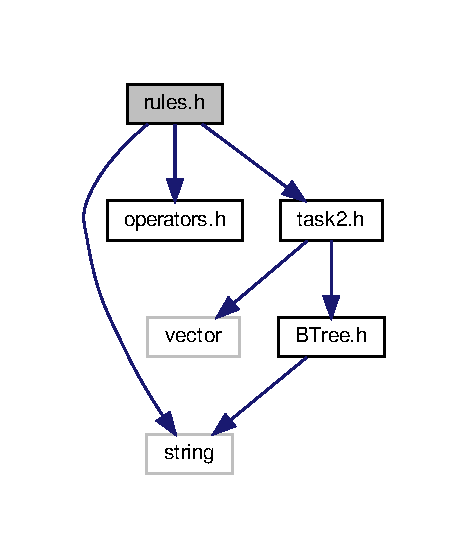
\includegraphics[width=224pt]{rules_8h__incl}
\end{center}
\end{figure}
This graph shows which files directly or indirectly include this file\+:\nopagebreak
\begin{figure}[H]
\begin{center}
\leavevmode
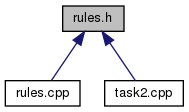
\includegraphics[width=214pt]{rules_8h__dep__incl}
\end{center}
\end{figure}
\subsection*{Namespaces}
\begin{DoxyCompactItemize}
\item 
 \mbox{\hyperlink{namespaceverbs}{verbs}}
\begin{DoxyCompactList}\small\item\em Defining verbs for ease of making changes if required. \end{DoxyCompactList}\item 
 \mbox{\hyperlink{namespacerule__literals}{rule\+\_\+literals}}
\begin{DoxyCompactList}\small\item\em Defining types of rules for ease of making changes if required. \end{DoxyCompactList}\end{DoxyCompactItemize}
\subsection*{Functions}
\begin{DoxyCompactItemize}
\item 
bool \mbox{\hyperlink{rules_8h_ad34f3b0deb1e94d6b1c44a2de9680972}{check\+\_\+validity}} (\mbox{\hyperlink{classProofLine}{Proof\+Line}} $\ast$newline)
\begin{DoxyCompactList}\small\item\em Checks validity of given \mbox{\hyperlink{classProofLine}{Proof\+Line}}. \end{DoxyCompactList}\item 
bool \mbox{\hyperlink{rules_8h_a3d9c86a35ee3da94e663c41d40ff279b}{check\+\_\+valid\+\_\+prem}} (\mbox{\hyperlink{classProofLine}{Proof\+Line}} $\ast$newline)
\begin{DoxyCompactList}\small\item\em Checks validity of given P\+R\+E\+M\+I\+SE \mbox{\hyperlink{classProofLine}{Proof\+Line}}. \end{DoxyCompactList}\item 
bool \mbox{\hyperlink{rules_8h_a118aab7800af68c5b32fa5e103c75741}{check\+\_\+valid\+\_\+and\+\_\+i}} (\mbox{\hyperlink{classProofLine}{Proof\+Line}} $\ast$newline)
\begin{DoxyCompactList}\small\item\em Checks validity of given A\+ND I\+N\+T\+R\+O\+D\+U\+C\+T\+I\+ON \mbox{\hyperlink{classProofLine}{Proof\+Line}}. \end{DoxyCompactList}\item 
bool \mbox{\hyperlink{rules_8h_abdc10668ade35c80f0fd187c837e1a77}{check\+\_\+valid\+\_\+and\+\_\+e1}} (\mbox{\hyperlink{classProofLine}{Proof\+Line}} $\ast$newline)
\begin{DoxyCompactList}\small\item\em Checks validity of given A\+ND E\+L\+I\+M\+I\+N\+A\+T\+I\+ON 1 \mbox{\hyperlink{classProofLine}{Proof\+Line}}. \end{DoxyCompactList}\item 
bool \mbox{\hyperlink{rules_8h_add6d4592664b8ce7ed7e02f8f76a9a2a}{check\+\_\+valid\+\_\+and\+\_\+e2}} (\mbox{\hyperlink{classProofLine}{Proof\+Line}} $\ast$newline)
\begin{DoxyCompactList}\small\item\em Checks validity of given A\+ND E\+L\+I\+M\+I\+N\+A\+T\+I\+ON 2 \mbox{\hyperlink{classProofLine}{Proof\+Line}}. \end{DoxyCompactList}\item 
bool \mbox{\hyperlink{rules_8h_a2a3a60e30b9b569cacc3e2f1ec08747a}{check\+\_\+valid\+\_\+or\+\_\+i1}} (\mbox{\hyperlink{classProofLine}{Proof\+Line}} $\ast$newline)
\begin{DoxyCompactList}\small\item\em Checks validity of given OR I\+N\+T\+R\+O\+D\+U\+C\+T\+I\+ON 1 \mbox{\hyperlink{classProofLine}{Proof\+Line}}. \end{DoxyCompactList}\item 
bool \mbox{\hyperlink{rules_8h_abe95433e64d9bc565b87ccd6161a5db9}{check\+\_\+valid\+\_\+or\+\_\+i2}} (\mbox{\hyperlink{classProofLine}{Proof\+Line}} $\ast$newline)
\begin{DoxyCompactList}\small\item\em Checks validity of given OR I\+N\+T\+R\+O\+D\+U\+C\+T\+I\+ON 2 \mbox{\hyperlink{classProofLine}{Proof\+Line}}. \end{DoxyCompactList}\item 
bool \mbox{\hyperlink{rules_8h_a0c6ca18751b18ba87a745683438fe31a}{check\+\_\+valid\+\_\+impl\+\_\+e}} (\mbox{\hyperlink{classProofLine}{Proof\+Line}} $\ast$newline)
\begin{DoxyCompactList}\small\item\em Checks validity of given I\+M\+P\+L\+I\+C\+A\+T\+I\+ON E\+L\+I\+M\+I\+N\+A\+T\+I\+ON \mbox{\hyperlink{classProofLine}{Proof\+Line}}. \end{DoxyCompactList}\item 
bool \mbox{\hyperlink{rules_8h_a067d8de671da3f3ce43054723e31d232}{check\+\_\+valid\+\_\+mt}} (\mbox{\hyperlink{classProofLine}{Proof\+Line}} $\ast$newline)
\begin{DoxyCompactList}\small\item\em Checks validity of given M\+O\+D\+US T\+O\+L\+L\+E\+NS \mbox{\hyperlink{classProofLine}{Proof\+Line}}. \end{DoxyCompactList}\end{DoxyCompactItemize}
\subsection*{Variables}
\begin{DoxyCompactItemize}
\item 
const char \mbox{\hyperlink{namespaceverbs_a160cd2b49b96eb11b6db907bf94b5c3a}{verbs\+::\+I\+N\+T\+RO}} \{\textquotesingle{}i\textquotesingle{}\}
\begin{DoxyCompactList}\small\item\em Defines I\+N\+T\+R\+O\+D\+U\+C\+T\+I\+ON. \end{DoxyCompactList}\item 
const char \mbox{\hyperlink{namespaceverbs_ae28355cc9321ebee9abcd23bb6e1b836}{verbs\+::\+E\+L\+IM}} \{\textquotesingle{}e\textquotesingle{}\}
\begin{DoxyCompactList}\small\item\em Defines E\+L\+I\+M\+I\+N\+A\+T\+I\+ON. \end{DoxyCompactList}\item 
const std\+::string \mbox{\hyperlink{namespacerule__literals_a28f9829b438b28638be8c82c450237e1}{rule\+\_\+literals\+::\+P\+R\+EM}} \{\char`\"{}P\char`\"{}\}
\begin{DoxyCompactList}\small\item\em $<$ Enables us to use A\+ND, OR, I\+M\+PL, N\+EG \end{DoxyCompactList}\item 
const std\+::string \mbox{\hyperlink{namespacerule__literals_a94631d6e4135b29c6bacb5cde1d9719b}{rule\+\_\+literals\+::\+A\+N\+D\+\_\+I}} \{A\+ND, \mbox{\hyperlink{namespaceverbs_a160cd2b49b96eb11b6db907bf94b5c3a}{verbs\+::\+I\+N\+T\+RO}}\}
\begin{DoxyCompactList}\small\item\em Defines A\+ND I\+N\+T\+R\+O\+D\+U\+C\+T\+I\+ON. \end{DoxyCompactList}\item 
const std\+::string \mbox{\hyperlink{namespacerule__literals_af7751bceefaea1ff69733140731b7770}{rule\+\_\+literals\+::\+A\+N\+D\+\_\+\+E1}} \{A\+ND, \mbox{\hyperlink{namespaceverbs_ae28355cc9321ebee9abcd23bb6e1b836}{verbs\+::\+E\+L\+IM}}, \textquotesingle{}1\textquotesingle{}\}
\begin{DoxyCompactList}\small\item\em Defines A\+ND E\+L\+I\+M\+I\+N\+A\+T\+I\+ON 1. \end{DoxyCompactList}\item 
const std\+::string \mbox{\hyperlink{namespacerule__literals_a0861b2e3104a4c1465d3dbbb362b5d10}{rule\+\_\+literals\+::\+A\+N\+D\+\_\+\+E2}} \{A\+ND, \mbox{\hyperlink{namespaceverbs_ae28355cc9321ebee9abcd23bb6e1b836}{verbs\+::\+E\+L\+IM}}, \textquotesingle{}2\textquotesingle{}\}
\begin{DoxyCompactList}\small\item\em Defines A\+ND E\+L\+I\+M\+I\+N\+A\+T\+I\+ON 2. \end{DoxyCompactList}\item 
const std\+::string \mbox{\hyperlink{namespacerule__literals_a0c61940a6e12e4ea3a41346b5b3c5870}{rule\+\_\+literals\+::\+O\+R\+\_\+\+I1}} \{OR, \mbox{\hyperlink{namespaceverbs_a160cd2b49b96eb11b6db907bf94b5c3a}{verbs\+::\+I\+N\+T\+RO}}, \textquotesingle{}1\textquotesingle{}\}
\begin{DoxyCompactList}\small\item\em Defines OR I\+N\+T\+R\+O\+D\+U\+C\+T\+I\+ON 1. \end{DoxyCompactList}\item 
const std\+::string \mbox{\hyperlink{namespacerule__literals_a2c1ef10ddec67801c44ea5b3e15ed133}{rule\+\_\+literals\+::\+O\+R\+\_\+\+I2}} \{OR, \mbox{\hyperlink{namespaceverbs_a160cd2b49b96eb11b6db907bf94b5c3a}{verbs\+::\+I\+N\+T\+RO}}, \textquotesingle{}2\textquotesingle{}\}
\begin{DoxyCompactList}\small\item\em Defines OR I\+N\+T\+R\+O\+D\+U\+C\+T\+I\+ON 2. \end{DoxyCompactList}\item 
const std\+::string \mbox{\hyperlink{namespacerule__literals_a51a002ead2192c49b9c6216c5fbe3b74}{rule\+\_\+literals\+::\+I\+M\+P\+L\+\_\+E}} \{I\+M\+PL, \mbox{\hyperlink{namespaceverbs_ae28355cc9321ebee9abcd23bb6e1b836}{verbs\+::\+E\+L\+IM}}\}
\begin{DoxyCompactList}\small\item\em Defines I\+M\+P\+L\+I\+ES E\+L\+I\+M\+I\+N\+A\+T\+I\+ON. \end{DoxyCompactList}\item 
const std\+::string \mbox{\hyperlink{namespacerule__literals_a056c3d0c0b701c07f444b7c5adfa8ff4}{rule\+\_\+literals\+::\+MT}} \{\char`\"{}MT\char`\"{}\}
\begin{DoxyCompactList}\small\item\em Defines M\+O\+D\+US T\+O\+L\+L\+E\+NS. \end{DoxyCompactList}\end{DoxyCompactItemize}


\subsection{Function Documentation}
\mbox{\Hypertarget{rules_8h_ad34f3b0deb1e94d6b1c44a2de9680972}\label{rules_8h_ad34f3b0deb1e94d6b1c44a2de9680972}} 
\index{rules.\+h@{rules.\+h}!check\+\_\+validity@{check\+\_\+validity}}
\index{check\+\_\+validity@{check\+\_\+validity}!rules.\+h@{rules.\+h}}
\subsubsection{\texorpdfstring{check\+\_\+validity()}{check\_validity()}}
{\footnotesize\ttfamily bool check\+\_\+validity (\begin{DoxyParamCaption}\item[{\mbox{\hyperlink{classProofLine}{Proof\+Line}} $\ast$}]{newline }\end{DoxyParamCaption})}



Checks validity of given \mbox{\hyperlink{classProofLine}{Proof\+Line}}. 

Complexity\+: O(1) 
\begin{DoxyParams}[1]{Parameters}
\mbox{\texttt{ in}}  & {\em newline} & Pointer to \mbox{\hyperlink{classProofLine}{Proof\+Line}} to be validated \\
\hline
\end{DoxyParams}
\begin{DoxyReturn}{Returns}
true if the \mbox{\hyperlink{classProofLine}{Proof\+Line}} is valid else false 
\end{DoxyReturn}
\mbox{\Hypertarget{rules_8h_a3d9c86a35ee3da94e663c41d40ff279b}\label{rules_8h_a3d9c86a35ee3da94e663c41d40ff279b}} 
\index{rules.\+h@{rules.\+h}!check\+\_\+valid\+\_\+prem@{check\+\_\+valid\+\_\+prem}}
\index{check\+\_\+valid\+\_\+prem@{check\+\_\+valid\+\_\+prem}!rules.\+h@{rules.\+h}}
\subsubsection{\texorpdfstring{check\+\_\+valid\+\_\+prem()}{check\_valid\_prem()}}
{\footnotesize\ttfamily bool check\+\_\+valid\+\_\+prem (\begin{DoxyParamCaption}\item[{\mbox{\hyperlink{classProofLine}{Proof\+Line}} $\ast$}]{newline }\end{DoxyParamCaption})}



Checks validity of given P\+R\+E\+M\+I\+SE \mbox{\hyperlink{classProofLine}{Proof\+Line}}. 

Complexity\+: O(1) 
\begin{DoxyParams}[1]{Parameters}
\mbox{\texttt{ in}}  & {\em newline} & Pointer to the P\+R\+E\+M\+I\+SE \mbox{\hyperlink{classProofLine}{Proof\+Line}} \\
\hline
\end{DoxyParams}
\begin{DoxyReturn}{Returns}
true if \mbox{\hyperlink{classProofLine}{Proof\+Line}} is a P\+R\+E\+M\+I\+SE else false 
\end{DoxyReturn}
\mbox{\Hypertarget{rules_8h_a118aab7800af68c5b32fa5e103c75741}\label{rules_8h_a118aab7800af68c5b32fa5e103c75741}} 
\index{rules.\+h@{rules.\+h}!check\+\_\+valid\+\_\+and\+\_\+i@{check\+\_\+valid\+\_\+and\+\_\+i}}
\index{check\+\_\+valid\+\_\+and\+\_\+i@{check\+\_\+valid\+\_\+and\+\_\+i}!rules.\+h@{rules.\+h}}
\subsubsection{\texorpdfstring{check\+\_\+valid\+\_\+and\+\_\+i()}{check\_valid\_and\_i()}}
{\footnotesize\ttfamily bool check\+\_\+valid\+\_\+and\+\_\+i (\begin{DoxyParamCaption}\item[{\mbox{\hyperlink{classProofLine}{Proof\+Line}} $\ast$}]{newline }\end{DoxyParamCaption})}



Checks validity of given A\+ND I\+N\+T\+R\+O\+D\+U\+C\+T\+I\+ON \mbox{\hyperlink{classProofLine}{Proof\+Line}}. 

Complexity\+: O(1) 
\begin{DoxyParams}[1]{Parameters}
\mbox{\texttt{ in}}  & {\em newline} & Pointer to the A\+ND I\+N\+T\+R\+O\+D\+U\+C\+T\+I\+ON \mbox{\hyperlink{classProofLine}{Proof\+Line}} \\
\hline
\end{DoxyParams}
\begin{DoxyReturn}{Returns}
true if the \mbox{\hyperlink{classProofLine}{Proof\+Line}} is valid else false 
\end{DoxyReturn}
\mbox{\Hypertarget{rules_8h_abdc10668ade35c80f0fd187c837e1a77}\label{rules_8h_abdc10668ade35c80f0fd187c837e1a77}} 
\index{rules.\+h@{rules.\+h}!check\+\_\+valid\+\_\+and\+\_\+e1@{check\+\_\+valid\+\_\+and\+\_\+e1}}
\index{check\+\_\+valid\+\_\+and\+\_\+e1@{check\+\_\+valid\+\_\+and\+\_\+e1}!rules.\+h@{rules.\+h}}
\subsubsection{\texorpdfstring{check\+\_\+valid\+\_\+and\+\_\+e1()}{check\_valid\_and\_e1()}}
{\footnotesize\ttfamily bool check\+\_\+valid\+\_\+and\+\_\+e1 (\begin{DoxyParamCaption}\item[{\mbox{\hyperlink{classProofLine}{Proof\+Line}} $\ast$}]{newline }\end{DoxyParamCaption})}



Checks validity of given A\+ND E\+L\+I\+M\+I\+N\+A\+T\+I\+ON 1 \mbox{\hyperlink{classProofLine}{Proof\+Line}}. 

Complexity\+: O(1) 
\begin{DoxyParams}[1]{Parameters}
\mbox{\texttt{ in}}  & {\em newline} & Pointer to the A\+ND E\+L\+I\+M\+I\+N\+A\+T\+I\+ON 1 \mbox{\hyperlink{classProofLine}{Proof\+Line}} \\
\hline
\end{DoxyParams}
\begin{DoxyReturn}{Returns}
true if the \mbox{\hyperlink{classProofLine}{Proof\+Line}} is valid else false 
\end{DoxyReturn}
\mbox{\Hypertarget{rules_8h_add6d4592664b8ce7ed7e02f8f76a9a2a}\label{rules_8h_add6d4592664b8ce7ed7e02f8f76a9a2a}} 
\index{rules.\+h@{rules.\+h}!check\+\_\+valid\+\_\+and\+\_\+e2@{check\+\_\+valid\+\_\+and\+\_\+e2}}
\index{check\+\_\+valid\+\_\+and\+\_\+e2@{check\+\_\+valid\+\_\+and\+\_\+e2}!rules.\+h@{rules.\+h}}
\subsubsection{\texorpdfstring{check\+\_\+valid\+\_\+and\+\_\+e2()}{check\_valid\_and\_e2()}}
{\footnotesize\ttfamily bool check\+\_\+valid\+\_\+and\+\_\+e2 (\begin{DoxyParamCaption}\item[{\mbox{\hyperlink{classProofLine}{Proof\+Line}} $\ast$}]{newline }\end{DoxyParamCaption})}



Checks validity of given A\+ND E\+L\+I\+M\+I\+N\+A\+T\+I\+ON 2 \mbox{\hyperlink{classProofLine}{Proof\+Line}}. 

Complexity\+: O(1) 
\begin{DoxyParams}[1]{Parameters}
\mbox{\texttt{ in}}  & {\em newline} & Pointer to the A\+ND E\+L\+I\+M\+I\+N\+A\+T\+I\+ON 2 \mbox{\hyperlink{classProofLine}{Proof\+Line}} \\
\hline
\end{DoxyParams}
\begin{DoxyReturn}{Returns}
true if the \mbox{\hyperlink{classProofLine}{Proof\+Line}} is valid else false 
\end{DoxyReturn}
\mbox{\Hypertarget{rules_8h_a2a3a60e30b9b569cacc3e2f1ec08747a}\label{rules_8h_a2a3a60e30b9b569cacc3e2f1ec08747a}} 
\index{rules.\+h@{rules.\+h}!check\+\_\+valid\+\_\+or\+\_\+i1@{check\+\_\+valid\+\_\+or\+\_\+i1}}
\index{check\+\_\+valid\+\_\+or\+\_\+i1@{check\+\_\+valid\+\_\+or\+\_\+i1}!rules.\+h@{rules.\+h}}
\subsubsection{\texorpdfstring{check\+\_\+valid\+\_\+or\+\_\+i1()}{check\_valid\_or\_i1()}}
{\footnotesize\ttfamily bool check\+\_\+valid\+\_\+or\+\_\+i1 (\begin{DoxyParamCaption}\item[{\mbox{\hyperlink{classProofLine}{Proof\+Line}} $\ast$}]{newline }\end{DoxyParamCaption})}



Checks validity of given OR I\+N\+T\+R\+O\+D\+U\+C\+T\+I\+ON 1 \mbox{\hyperlink{classProofLine}{Proof\+Line}}. 

Complexity\+: O(1) 
\begin{DoxyParams}[1]{Parameters}
\mbox{\texttt{ in}}  & {\em newline} & Pointer to the OR I\+N\+T\+R\+O\+D\+U\+C\+T\+I\+ON 1 \mbox{\hyperlink{classProofLine}{Proof\+Line}} \\
\hline
\end{DoxyParams}
\begin{DoxyReturn}{Returns}
true if the \mbox{\hyperlink{classProofLine}{Proof\+Line}} is valid else false 
\end{DoxyReturn}
\mbox{\Hypertarget{rules_8h_abe95433e64d9bc565b87ccd6161a5db9}\label{rules_8h_abe95433e64d9bc565b87ccd6161a5db9}} 
\index{rules.\+h@{rules.\+h}!check\+\_\+valid\+\_\+or\+\_\+i2@{check\+\_\+valid\+\_\+or\+\_\+i2}}
\index{check\+\_\+valid\+\_\+or\+\_\+i2@{check\+\_\+valid\+\_\+or\+\_\+i2}!rules.\+h@{rules.\+h}}
\subsubsection{\texorpdfstring{check\+\_\+valid\+\_\+or\+\_\+i2()}{check\_valid\_or\_i2()}}
{\footnotesize\ttfamily bool check\+\_\+valid\+\_\+or\+\_\+i2 (\begin{DoxyParamCaption}\item[{\mbox{\hyperlink{classProofLine}{Proof\+Line}} $\ast$}]{newline }\end{DoxyParamCaption})}



Checks validity of given OR I\+N\+T\+R\+O\+D\+U\+C\+T\+I\+ON 2 \mbox{\hyperlink{classProofLine}{Proof\+Line}}. 

Complexity\+: O(1) 
\begin{DoxyParams}[1]{Parameters}
\mbox{\texttt{ in}}  & {\em newline} & Pointer to the OR I\+N\+T\+R\+O\+D\+U\+C\+T\+I\+ON 2 \mbox{\hyperlink{classProofLine}{Proof\+Line}} \\
\hline
\end{DoxyParams}
\begin{DoxyReturn}{Returns}
true if the \mbox{\hyperlink{classProofLine}{Proof\+Line}} is valid else false 
\end{DoxyReturn}
\mbox{\Hypertarget{rules_8h_a0c6ca18751b18ba87a745683438fe31a}\label{rules_8h_a0c6ca18751b18ba87a745683438fe31a}} 
\index{rules.\+h@{rules.\+h}!check\+\_\+valid\+\_\+impl\+\_\+e@{check\+\_\+valid\+\_\+impl\+\_\+e}}
\index{check\+\_\+valid\+\_\+impl\+\_\+e@{check\+\_\+valid\+\_\+impl\+\_\+e}!rules.\+h@{rules.\+h}}
\subsubsection{\texorpdfstring{check\+\_\+valid\+\_\+impl\+\_\+e()}{check\_valid\_impl\_e()}}
{\footnotesize\ttfamily bool check\+\_\+valid\+\_\+impl\+\_\+e (\begin{DoxyParamCaption}\item[{\mbox{\hyperlink{classProofLine}{Proof\+Line}} $\ast$}]{newline }\end{DoxyParamCaption})}



Checks validity of given I\+M\+P\+L\+I\+C\+A\+T\+I\+ON E\+L\+I\+M\+I\+N\+A\+T\+I\+ON \mbox{\hyperlink{classProofLine}{Proof\+Line}}. 

Complexity\+: O(1) 
\begin{DoxyParams}[1]{Parameters}
\mbox{\texttt{ in}}  & {\em newline} & Pointer to the I\+M\+P\+L\+I\+C\+A\+T\+I\+ON E\+L\+I\+M\+I\+N\+A\+T\+I\+ON \mbox{\hyperlink{classProofLine}{Proof\+Line}} \\
\hline
\end{DoxyParams}
\begin{DoxyReturn}{Returns}
true if the \mbox{\hyperlink{classProofLine}{Proof\+Line}} is valid else false 
\end{DoxyReturn}
\mbox{\Hypertarget{rules_8h_a067d8de671da3f3ce43054723e31d232}\label{rules_8h_a067d8de671da3f3ce43054723e31d232}} 
\index{rules.\+h@{rules.\+h}!check\+\_\+valid\+\_\+mt@{check\+\_\+valid\+\_\+mt}}
\index{check\+\_\+valid\+\_\+mt@{check\+\_\+valid\+\_\+mt}!rules.\+h@{rules.\+h}}
\subsubsection{\texorpdfstring{check\+\_\+valid\+\_\+mt()}{check\_valid\_mt()}}
{\footnotesize\ttfamily bool check\+\_\+valid\+\_\+mt (\begin{DoxyParamCaption}\item[{\mbox{\hyperlink{classProofLine}{Proof\+Line}} $\ast$}]{newline }\end{DoxyParamCaption})}



Checks validity of given M\+O\+D\+US T\+O\+L\+L\+E\+NS \mbox{\hyperlink{classProofLine}{Proof\+Line}}. 

Complexity\+: O(1) 
\begin{DoxyParams}[1]{Parameters}
\mbox{\texttt{ in}}  & {\em newline} & Pointer to the M\+O\+D\+US T\+O\+L\+L\+E\+NS \mbox{\hyperlink{classProofLine}{Proof\+Line}} \\
\hline
\end{DoxyParams}
\begin{DoxyReturn}{Returns}
true if the \mbox{\hyperlink{classProofLine}{Proof\+Line}} is valid else false 
\end{DoxyReturn}

\hypertarget{task1_8cpp}{}\section{task1.\+cpp File Reference}
\label{task1_8cpp}\index{task1.\+cpp@{task1.\+cpp}}
{\ttfamily \#include $<$stack$>$}\newline
{\ttfamily \#include $<$string$>$}\newline
{\ttfamily \#include \char`\"{}operators.\+h\char`\"{}}\newline
{\ttfamily \#include \char`\"{}task1.\+h\char`\"{}}\newline
Include dependency graph for task1.\+cpp\+:
% FIG 0
\subsection*{Functions}
\begin{DoxyCompactItemize}
\item 
string \hyperlink{task1_8cpp_a1cec0e0fc4a01011912b6220bbe8cb68}{infix\+\_\+to\+\_\+postfix} (string infix\+\_\+exp)
\item 
\hyperlink{classBTree}{B\+Tree} $\ast$ \hyperlink{task1_8cpp_ad88f7bb236ca2d68cff798a6f554352f}{postfix\+\_\+to\+\_\+parse\+\_\+tree} (string $\ast$postfix)
\item 
string \hyperlink{task1_8cpp_aa808b56f8dad579fdb383b1d7bfb0620}{parse\+\_\+tree\+\_\+to\+\_\+infix} (\hyperlink{classBTree}{B\+Tree} $\ast$root)
\end{DoxyCompactItemize}


\subsection{Function Documentation}
\mbox{\Hypertarget{task1_8cpp_a1cec0e0fc4a01011912b6220bbe8cb68}\label{task1_8cpp_a1cec0e0fc4a01011912b6220bbe8cb68}} 
\index{task1.\+cpp@{task1.\+cpp}!infix\+\_\+to\+\_\+postfix@{infix\+\_\+to\+\_\+postfix}}
\index{infix\+\_\+to\+\_\+postfix@{infix\+\_\+to\+\_\+postfix}!task1.\+cpp@{task1.\+cpp}}
\subsubsection{\texorpdfstring{infix\+\_\+to\+\_\+postfix()}{infix\_to\_postfix()}}
{\footnotesize\ttfamily string infix\+\_\+to\+\_\+postfix (\begin{DoxyParamCaption}\item[{string}]{infix\+\_\+exp }\end{DoxyParamCaption})}

\mbox{\Hypertarget{task1_8cpp_aa808b56f8dad579fdb383b1d7bfb0620}\label{task1_8cpp_aa808b56f8dad579fdb383b1d7bfb0620}} 
\index{task1.\+cpp@{task1.\+cpp}!parse\+\_\+tree\+\_\+to\+\_\+infix@{parse\+\_\+tree\+\_\+to\+\_\+infix}}
\index{parse\+\_\+tree\+\_\+to\+\_\+infix@{parse\+\_\+tree\+\_\+to\+\_\+infix}!task1.\+cpp@{task1.\+cpp}}
\subsubsection{\texorpdfstring{parse\+\_\+tree\+\_\+to\+\_\+infix()}{parse\_tree\_to\_infix()}}
{\footnotesize\ttfamily string parse\+\_\+tree\+\_\+to\+\_\+infix (\begin{DoxyParamCaption}\item[{\hyperlink{classBTree}{B\+Tree} $\ast$}]{root }\end{DoxyParamCaption})}


\begin{DoxyParams}{Parameters}
{\em root} & It is the root of the parse tree which we want to convert to infix form \\
\hline
\end{DoxyParams}
\begin{DoxyReturn}{Returns}
A string containing the original infix expression through which the parse tree was generated 
\end{DoxyReturn}
\mbox{\Hypertarget{task1_8cpp_ad88f7bb236ca2d68cff798a6f554352f}\label{task1_8cpp_ad88f7bb236ca2d68cff798a6f554352f}} 
\index{task1.\+cpp@{task1.\+cpp}!postfix\+\_\+to\+\_\+parse\+\_\+tree@{postfix\+\_\+to\+\_\+parse\+\_\+tree}}
\index{postfix\+\_\+to\+\_\+parse\+\_\+tree@{postfix\+\_\+to\+\_\+parse\+\_\+tree}!task1.\+cpp@{task1.\+cpp}}
\subsubsection{\texorpdfstring{postfix\+\_\+to\+\_\+parse\+\_\+tree()}{postfix\_to\_parse\_tree()}}
{\footnotesize\ttfamily \hyperlink{classBTree}{B\+Tree}$\ast$ postfix\+\_\+to\+\_\+parse\+\_\+tree (\begin{DoxyParamCaption}\item[{string $\ast$}]{postfix }\end{DoxyParamCaption})}


\hypertarget{task1_8h}{}\section{task1.\+h File Reference}
\label{task1_8h}\index{task1.\+h@{task1.\+h}}
{\ttfamily \#include \char`\"{}B\+Tree.\+h\char`\"{}}\newline
Include dependency graph for task1.\+h\+:\nopagebreak
\begin{figure}[H]
\begin{center}
\leavevmode
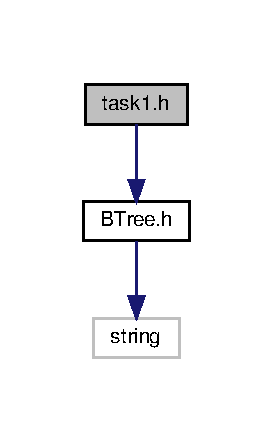
\includegraphics[width=131pt]{task1_8h__incl}
\end{center}
\end{figure}
This graph shows which files directly or indirectly include this file\+:\nopagebreak
\begin{figure}[H]
\begin{center}
\leavevmode
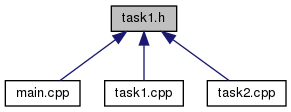
\includegraphics[width=291pt]{task1_8h__dep__incl}
\end{center}
\end{figure}
\subsection*{Functions}
\begin{DoxyCompactItemize}
\item 
std\+::string \mbox{\hyperlink{task1_8h_a2dbc497c79c44fc43579cedee34296e8}{infix\+\_\+to\+\_\+postfix}} (std\+::string infix\+\_\+exp)
\begin{DoxyCompactList}\small\item\em Converts the infix expression to postfix. \end{DoxyCompactList}\item 
\mbox{\hyperlink{classBTree}{B\+Tree}} $\ast$ \mbox{\hyperlink{task1_8h_a628ffca8bc269400217fa849038b6684}{postfix\+\_\+to\+\_\+parse\+\_\+tree}} (std\+::string $\ast$postfix)
\begin{DoxyCompactList}\small\item\em Generates a binary tree using given postfix expression. \end{DoxyCompactList}\item 
std\+::string \mbox{\hyperlink{task1_8h_a9804f1d5620990cac8ac016f30cb6f4f}{parse\+\_\+tree\+\_\+to\+\_\+infix}} (\mbox{\hyperlink{classBTree}{B\+Tree}} $\ast$root)
\begin{DoxyCompactList}\small\item\em Traverses a given tree to produce corresponding infix expression. \end{DoxyCompactList}\end{DoxyCompactItemize}


\subsection{Function Documentation}
\mbox{\Hypertarget{task1_8h_a2dbc497c79c44fc43579cedee34296e8}\label{task1_8h_a2dbc497c79c44fc43579cedee34296e8}} 
\index{task1.\+h@{task1.\+h}!infix\+\_\+to\+\_\+postfix@{infix\+\_\+to\+\_\+postfix}}
\index{infix\+\_\+to\+\_\+postfix@{infix\+\_\+to\+\_\+postfix}!task1.\+h@{task1.\+h}}
\subsubsection{\texorpdfstring{infix\+\_\+to\+\_\+postfix()}{infix\_to\_postfix()}}
{\footnotesize\ttfamily std\+::string infix\+\_\+to\+\_\+postfix (\begin{DoxyParamCaption}\item[{std\+::string}]{infix\+\_\+exp }\end{DoxyParamCaption})}



Converts the infix expression to postfix. 

Complexity\+: O(number of characters in infix expression) 
\begin{DoxyParams}[1]{Parameters}
\mbox{\texttt{ in}}  & {\em infix\+\_\+exp} & The user-\/given string expression in infix form \\
\hline
\end{DoxyParams}
\begin{DoxyReturn}{Returns}
A string in postfix form 
\end{DoxyReturn}
\mbox{\Hypertarget{task1_8h_a628ffca8bc269400217fa849038b6684}\label{task1_8h_a628ffca8bc269400217fa849038b6684}} 
\index{task1.\+h@{task1.\+h}!postfix\+\_\+to\+\_\+parse\+\_\+tree@{postfix\+\_\+to\+\_\+parse\+\_\+tree}}
\index{postfix\+\_\+to\+\_\+parse\+\_\+tree@{postfix\+\_\+to\+\_\+parse\+\_\+tree}!task1.\+h@{task1.\+h}}
\subsubsection{\texorpdfstring{postfix\+\_\+to\+\_\+parse\+\_\+tree()}{postfix\_to\_parse\_tree()}}
{\footnotesize\ttfamily \mbox{\hyperlink{classBTree}{B\+Tree}} $\ast$ postfix\+\_\+to\+\_\+parse\+\_\+tree (\begin{DoxyParamCaption}\item[{std\+::string $\ast$}]{postfix }\end{DoxyParamCaption})}



Generates a binary tree using given postfix expression. 

\begin{DoxyWarning}{Warning}
This function modifies the postfix string it takes as argument!
\end{DoxyWarning}
Complexity\+: O(number of characters in postfix expression) 
\begin{DoxyParams}[1]{Parameters}
\mbox{\texttt{ in,out}}  & {\em postfix} & Postfix expression which we want to parse \\
\hline
\end{DoxyParams}
\begin{DoxyReturn}{Returns}
Root of the binary tree generated 
\end{DoxyReturn}
\mbox{\Hypertarget{task1_8h_a9804f1d5620990cac8ac016f30cb6f4f}\label{task1_8h_a9804f1d5620990cac8ac016f30cb6f4f}} 
\index{task1.\+h@{task1.\+h}!parse\+\_\+tree\+\_\+to\+\_\+infix@{parse\+\_\+tree\+\_\+to\+\_\+infix}}
\index{parse\+\_\+tree\+\_\+to\+\_\+infix@{parse\+\_\+tree\+\_\+to\+\_\+infix}!task1.\+h@{task1.\+h}}
\subsubsection{\texorpdfstring{parse\+\_\+tree\+\_\+to\+\_\+infix()}{parse\_tree\_to\_infix()}}
{\footnotesize\ttfamily std\+::string parse\+\_\+tree\+\_\+to\+\_\+infix (\begin{DoxyParamCaption}\item[{\mbox{\hyperlink{classBTree}{B\+Tree}} $\ast$}]{root }\end{DoxyParamCaption})}



Traverses a given tree to produce corresponding infix expression. 

Complexity\+: O(number of nodes in parse tree) 
\begin{DoxyParams}[1]{Parameters}
\mbox{\texttt{ in}}  & {\em root} & Root of binary tree to be traversed \\
\hline
\end{DoxyParams}
\begin{DoxyReturn}{Returns}
A string of infix expression of binary tree 
\end{DoxyReturn}

\hypertarget{task2_8cpp}{}\section{task2.\+cpp File Reference}
\label{task2_8cpp}\index{task2.\+cpp@{task2.\+cpp}}
{\ttfamily \#include $<$iostream$>$}\newline
{\ttfamily \#include $<$sstream$>$}\newline
{\ttfamily \#include $<$string$>$}\newline
{\ttfamily \#include $<$vector$>$}\newline
{\ttfamily \#include \char`\"{}rules.\+h\char`\"{}}\newline
{\ttfamily \#include \char`\"{}task1.\+h\char`\"{}}\newline
{\ttfamily \#include \char`\"{}task2.\+h\char`\"{}}\newline
Include dependency graph for task2.\+cpp\+:
% FIG 0
\subsection*{Functions}
\begin{DoxyCompactItemize}
\item 
\hyperlink{classProofLine}{Proof\+Line} $\ast$ \hyperlink{task2_8cpp_a3b63433afe31ee90fd747077e95590ba}{parse\+\_\+line} (string s, int line\+\_\+num, vector$<$ \hyperlink{classProofLine}{Proof\+Line} $\ast$$>$ prev\+\_\+lines)
\item 
void \hyperlink{task2_8cpp_a43022f1f1f94d244fad4a528ef0a8726}{validate\+\_\+proof} ()
\end{DoxyCompactItemize}


\subsection{Function Documentation}
\mbox{\Hypertarget{task2_8cpp_a3b63433afe31ee90fd747077e95590ba}\label{task2_8cpp_a3b63433afe31ee90fd747077e95590ba}} 
\index{task2.\+cpp@{task2.\+cpp}!parse\+\_\+line@{parse\+\_\+line}}
\index{parse\+\_\+line@{parse\+\_\+line}!task2.\+cpp@{task2.\+cpp}}
\subsubsection{\texorpdfstring{parse\+\_\+line()}{parse\_line()}}
{\footnotesize\ttfamily \hyperlink{classProofLine}{Proof\+Line}$\ast$ parse\+\_\+line (\begin{DoxyParamCaption}\item[{string}]{s,  }\item[{int}]{line\+\_\+num,  }\item[{vector$<$ \hyperlink{classProofLine}{Proof\+Line} $\ast$$>$}]{prev\+\_\+lines }\end{DoxyParamCaption})}

\mbox{\Hypertarget{task2_8cpp_a43022f1f1f94d244fad4a528ef0a8726}\label{task2_8cpp_a43022f1f1f94d244fad4a528ef0a8726}} 
\index{task2.\+cpp@{task2.\+cpp}!validate\+\_\+proof@{validate\+\_\+proof}}
\index{validate\+\_\+proof@{validate\+\_\+proof}!task2.\+cpp@{task2.\+cpp}}
\subsubsection{\texorpdfstring{validate\+\_\+proof()}{validate\_proof()}}
{\footnotesize\ttfamily void validate\+\_\+proof (\begin{DoxyParamCaption}{ }\end{DoxyParamCaption})}


\hypertarget{task2_8h}{}\section{task2.\+h File Reference}
\label{task2_8h}\index{task2.\+h@{task2.\+h}}
{\ttfamily \#include $<$vector$>$}\newline
{\ttfamily \#include \char`\"{}B\+Tree.\+h\char`\"{}}\newline
Include dependency graph for task2.\+h\+:\nopagebreak
\begin{figure}[H]
\begin{center}
\leavevmode
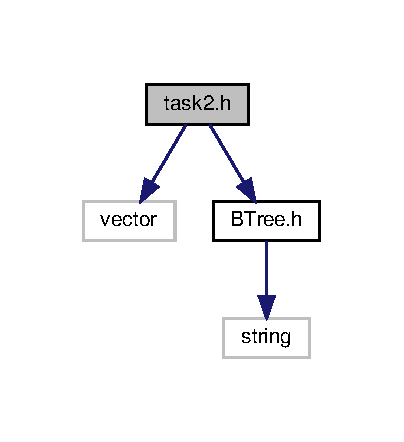
\includegraphics[width=194pt]{task2_8h__incl}
\end{center}
\end{figure}
This graph shows which files directly or indirectly include this file\+:\nopagebreak
\begin{figure}[H]
\begin{center}
\leavevmode
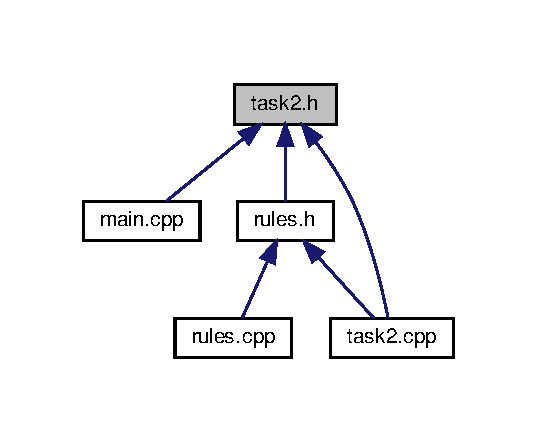
\includegraphics[width=258pt]{task2_8h__dep__incl}
\end{center}
\end{figure}
\subsection*{Classes}
\begin{DoxyCompactItemize}
\item 
class \mbox{\hyperlink{classProofLine}{Proof\+Line}}
\begin{DoxyCompactList}\small\item\em Class containing segregated information about a \mbox{\hyperlink{classProofLine}{Proof\+Line}}. \end{DoxyCompactList}\end{DoxyCompactItemize}
\subsection*{Functions}
\begin{DoxyCompactItemize}
\item 
\mbox{\hyperlink{classProofLine}{Proof\+Line}} $\ast$ \mbox{\hyperlink{task2_8h_a6d1300f474077a1440e6d8d2406a3d97}{parse\+\_\+line}} (std\+::string s, int line\+\_\+num, std\+::vector$<$ \mbox{\hyperlink{classProofLine}{Proof\+Line}} $\ast$$>$ prev\+\_\+lines)
\begin{DoxyCompactList}\small\item\em Makes new \mbox{\hyperlink{classProofLine}{Proof\+Line}} object using the input string. \end{DoxyCompactList}\item 
void \mbox{\hyperlink{task2_8h_a43022f1f1f94d244fad4a528ef0a8726}{validate\+\_\+proof}} ()
\begin{DoxyCompactList}\small\item\em Checks validity of user-\/given proof. \end{DoxyCompactList}\end{DoxyCompactItemize}


\subsection{Function Documentation}
\mbox{\Hypertarget{task2_8h_a6d1300f474077a1440e6d8d2406a3d97}\label{task2_8h_a6d1300f474077a1440e6d8d2406a3d97}} 
\index{task2.\+h@{task2.\+h}!parse\+\_\+line@{parse\+\_\+line}}
\index{parse\+\_\+line@{parse\+\_\+line}!task2.\+h@{task2.\+h}}
\subsubsection{\texorpdfstring{parse\+\_\+line()}{parse\_line()}}
{\footnotesize\ttfamily \mbox{\hyperlink{classProofLine}{Proof\+Line}} $\ast$ parse\+\_\+line (\begin{DoxyParamCaption}\item[{std\+::string}]{s,  }\item[{int}]{line\+\_\+num,  }\item[{std\+::vector$<$ \mbox{\hyperlink{classProofLine}{Proof\+Line}} $\ast$$>$}]{prev\+\_\+lines }\end{DoxyParamCaption})}



Makes new \mbox{\hyperlink{classProofLine}{Proof\+Line}} object using the input string. 


\begin{DoxyParams}[1]{Parameters}
\mbox{\texttt{ in}}  & {\em s} & Input string obtained from user \\
\hline
\mbox{\texttt{ in}}  & {\em line\+\_\+num} & Line number of current \mbox{\hyperlink{classProofLine}{Proof\+Line}} \\
\hline
\mbox{\texttt{ in}}  & {\em prev\+\_\+lines} & Vector containing all previous \mbox{\hyperlink{classProofLine}{Proof\+Line}} pointers \\
\hline
\end{DoxyParams}
\begin{DoxyReturn}{Returns}
Pointer to newly created \mbox{\hyperlink{classProofLine}{Proof\+Line}} object 
\end{DoxyReturn}
\mbox{\Hypertarget{task2_8h_a43022f1f1f94d244fad4a528ef0a8726}\label{task2_8h_a43022f1f1f94d244fad4a528ef0a8726}} 
\index{task2.\+h@{task2.\+h}!validate\+\_\+proof@{validate\+\_\+proof}}
\index{validate\+\_\+proof@{validate\+\_\+proof}!task2.\+h@{task2.\+h}}
\subsubsection{\texorpdfstring{validate\+\_\+proof()}{validate\_proof()}}
{\footnotesize\ttfamily void validate\+\_\+proof (\begin{DoxyParamCaption}{ }\end{DoxyParamCaption})}



Checks validity of user-\/given proof. 


%--- End generated contents ---

% Index
\backmatter
\newpage
\phantomsection
\clearemptydoublepage
\addcontentsline{toc}{chapter}{Index}
\printindex

\end{document}
